\chapter{Espacios Vectoriales}

El concepto de espacio vectorial generaliza las propiedades que tienen las operaciones de suma y producto por escalares  para los vectores de $\mathbb{R}^2$ y $\mathbb{R}^3$. Abordaremos en este capítulo la estructura de espacio vectorial, objeto básico de estudio del Álgebra Lineal. A sus elementos se los denomina vectores, independientemente de su naturaleza.

\bigskip


\section{Definición de espacio vectorial. Ejemplos  }\label{intro}


El conjunto de los números reales y el conjunto de los números complejos, con los cuales ya se trabajó, tienen propiedades similares. En ambos conjuntos pueden definirse dos operaciones $+$ y $.$ que satisfacen ciertas propiedades y reciben el nombre de  \textit{cuerpo}. Trabajaremos tanto con el cuerpo de los reales,  $\mathbb{R}$ como con el cuerpo de los complejos  $\mathbb{C}$, denotándolos por K.
Al estudiar vectores en el plano y en el espacio, se ha definido la \textit{suma de vectores} y la \textit{multiplicación por un número real}, y se vieron las propiedades que satisfacían. También para el conjunto de polinomios. 
Cuando en varios conjuntos distintos aparecen estructuras similares es conveniente axiomatizar éstas y darles un nombre al ente resultante, con la ventaja que estudiando esta estructura, quedan estudiadas todas las estructuras que en ella se encuadran. Cuando en un conjunto se da una estructura similar a la de los ejemplos anteriores, se dice que se tiene un \textit{espacio vectorial}.

\bigskip

\bigskip
 

\bigskip


\begin{definition}\index{Espacio Vectorial}
    {Un conjunto $V$, cuyos elementos se denotan mediante $\vec{u}$, $\vec{v}$, $\vec{w}$, se dice que es un \textit{espacio vectorial} sobre el cuerpo $K$, si en él se han definido dos operaciones: la \textit{suma}, de manera que a cada par de elementos $\vec{u}$ y $\vec{v}$ de $V$ se le hace corresponder el elemento $\vec{u}+\vec{v}$ de $V$, denominado suma de $\vec{u}$ y $\vec{v}$, y la \textit{multiplicación por escalares}, de manera que a todo elemento $\vec{u}$ de $V$  y a todo elemento $a$ de $K$ se le hace corresponder el elemento $a\vec{u}$ de $V$, y se satisfacen las siguientes propiedades:

\bigskip

%\vskip0.5cm

\begin{enumerate}
%\item[]\textbf{EJEMPLO 1:}


\item Conmutativa $~\vec{u}~ + ~\vec{v}~ = ~\vec{v}~ + ~\vec{u}~$ $~~\forall$ $\vec{u}$ y $\vec{v}$ $\in$ $V$.

\item Asociativa $~\vec{u}~ + (~\vec{v}~+  ~\vec{w}~)= (~\vec{u}~+  ~\vec{v}~) + ~\vec{w}~$,$~~\forall$ $\vec{u}$,  $\vec{v}$ y $\vec{w}$  $\in$ $V$. 
\item Existe un elemento de $V$, designado por $\vec{0}$ y denominado \textit{elemento neutro}, tal que 
$~\vec{u}~ + ~\vec{0}~ = ~\vec{u}~$ $\forall$ $\vec{u}$ $\in$ $V$.

\item Para todo elemento $\vec{u}$ $\in$ $V$, existe un elemento designado por $-\vec{u}$ y denominado \textit{elemento opuesto} de $\vec{u}$, tal que 
$~\vec{u}~ + ~(-\vec{u})~ = ~\vec{0}$

\item $1~\vec{u}~ =~\vec{u}~$ $\forall$ $\vec{u}$ $\in$ $V$, donde $1$ denota el elemento unidad del cuerpo  $K$. 

\item $a(b~\vec{u}~) =(ab)~\vec{u}~$ $~~\forall$ $\vec{u}$ $\in$ $V$, y $~~\forall$ $a$ y $b$ $  \in K$.
\item $(a+b)~\vec{u}~ =a~\vec{u}~+b~\vec{u}~ $ $\forall$ $\vec{u}$ $\in$ $V$, y todo $a$ y $b$ $\in$ K.
\item $a(~\vec{u}~+~\vec{v}~) =a~\vec{u}~+a~\vec{v}~ $ $\forall$ $\vec{u}$, $\vec{v}$ $\in$ $V$, y $\forall$ $a$ $\in$ K.

\end{enumerate}}
\end{definition}

\bigskip

\bigskip

En la Figura  \ref{fig:my_label} se muestra la propiedad conmutativa $1$.

%\begin{tikzpicture}[scale=1.5]
    % Draw axes
    %\draw [<->,thick] (0,2) node (yaxis) [above] {$y$}
        %|- (3,0) node (xaxis) [right] {$x$};
    % Draw two intersecting lines
    %\draw (0,0) coordinate (a_1) -- (2,1.8) coordinate (a_2);
    %\draw (0,1.5) coordinate (b_1) -- (2.5,0) coordinate (b_2);
    % Calculate the intersection of the lines a_1 -- a_2 and b_1 -- b_2
    % and store the coordinate in c.
    %\coordinate (c) at (intersection of a_1--a_2 and b_1--b_2);
    % Draw lines indicating intersection with y and x axis. Here we use
    % the perpendicular coordinate system
    %\draw[dashed] (yaxis |- c) node[left] {$y'$}
       % -| (xaxis -| c) node[below] {$x'$};
    % Draw a dot to indicate intersection point
    %\fill[red] (c) circle (2pt);
%\end{tikzpicture}

%\begin{tikzpicture} % ejes
%\draw[thin, blue] (0,0) -- (0,2) node (yaxis) [above] {$z$};
%\draw[thin, blue] (0,0) -- (2,0)  node (xaxis) [above] {$y$};
% segmento
%\draw[thin, blue]
%(0,0) -- (-1,-1) node (zaxis) [above] {$x$};
%\end{tikzpicture}


%\vskip0.5cm
%\tikzset{ % Lista de opciones de nodo
% opción draw = color borde
% opacity = porcentaje transparencia
% opción fill = color relleno
%opciones/.style={%
%draw= red!50!black!50,
%top color = white,
%bottom color = red!50!black!20,
%fill opacity = 0.6,
%rectangle, font=\small\bf\sffamily}
%}
%\begin{center}
%\begin{tikzpicture}
%\draw[draw= yellow!30,fill=yellow!30] (0,0) rectangle(2,2);
%\node[draw=black,rectangle, anchor=center] at (1,1) {$\bullet$};
%\node[opciones, anchor=south east] at (1,1) {ancla en el sur-este};
%\node[opciones, anchor=north west] at (1,1) {ancla en el norte-oeste};
%\end{tikzpicture}
%\caption{figure}{Nodos rectangular con anclaje en el sureste y noroeste}
%\end{center}
%\begin{tikzpicture}
%\draw[thick,->] (0,0,0) -- (1,0,0) %node[anchor=north east]{$x$};
%\draw[thick,->] (0,0,0) -- (0,1,0) node[anchor=north west]{$y$};
%\draw[thick,->] (0,0,0) -- (0,0,1) node[anchor=south]{$z$};
%\end{tikzpicture}

\begin{figure}
    \centering
    %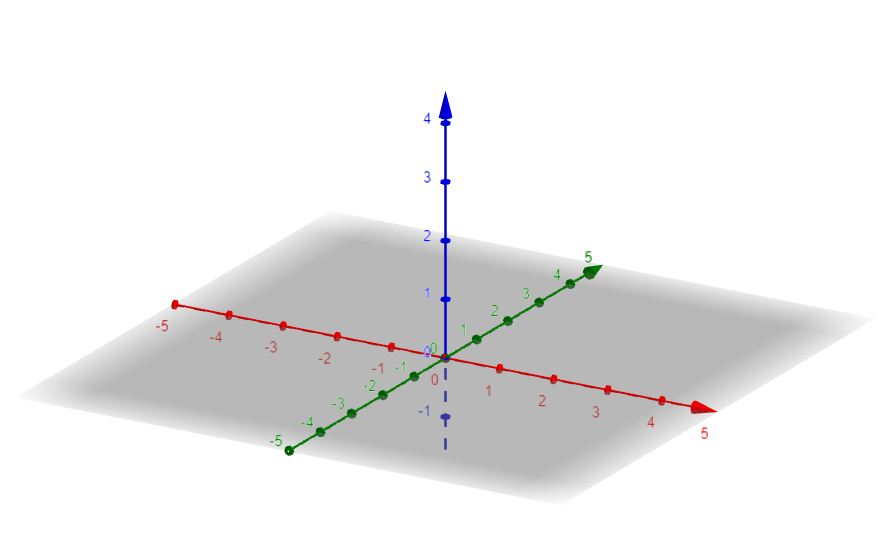
\includegraphics[width=0.60\textwidth]{Pictures/geogebra-export.png}
    %\caption{Caption}
    \label{fig:my_label}
\end{figure}
\begin{figure}
    \centering
    %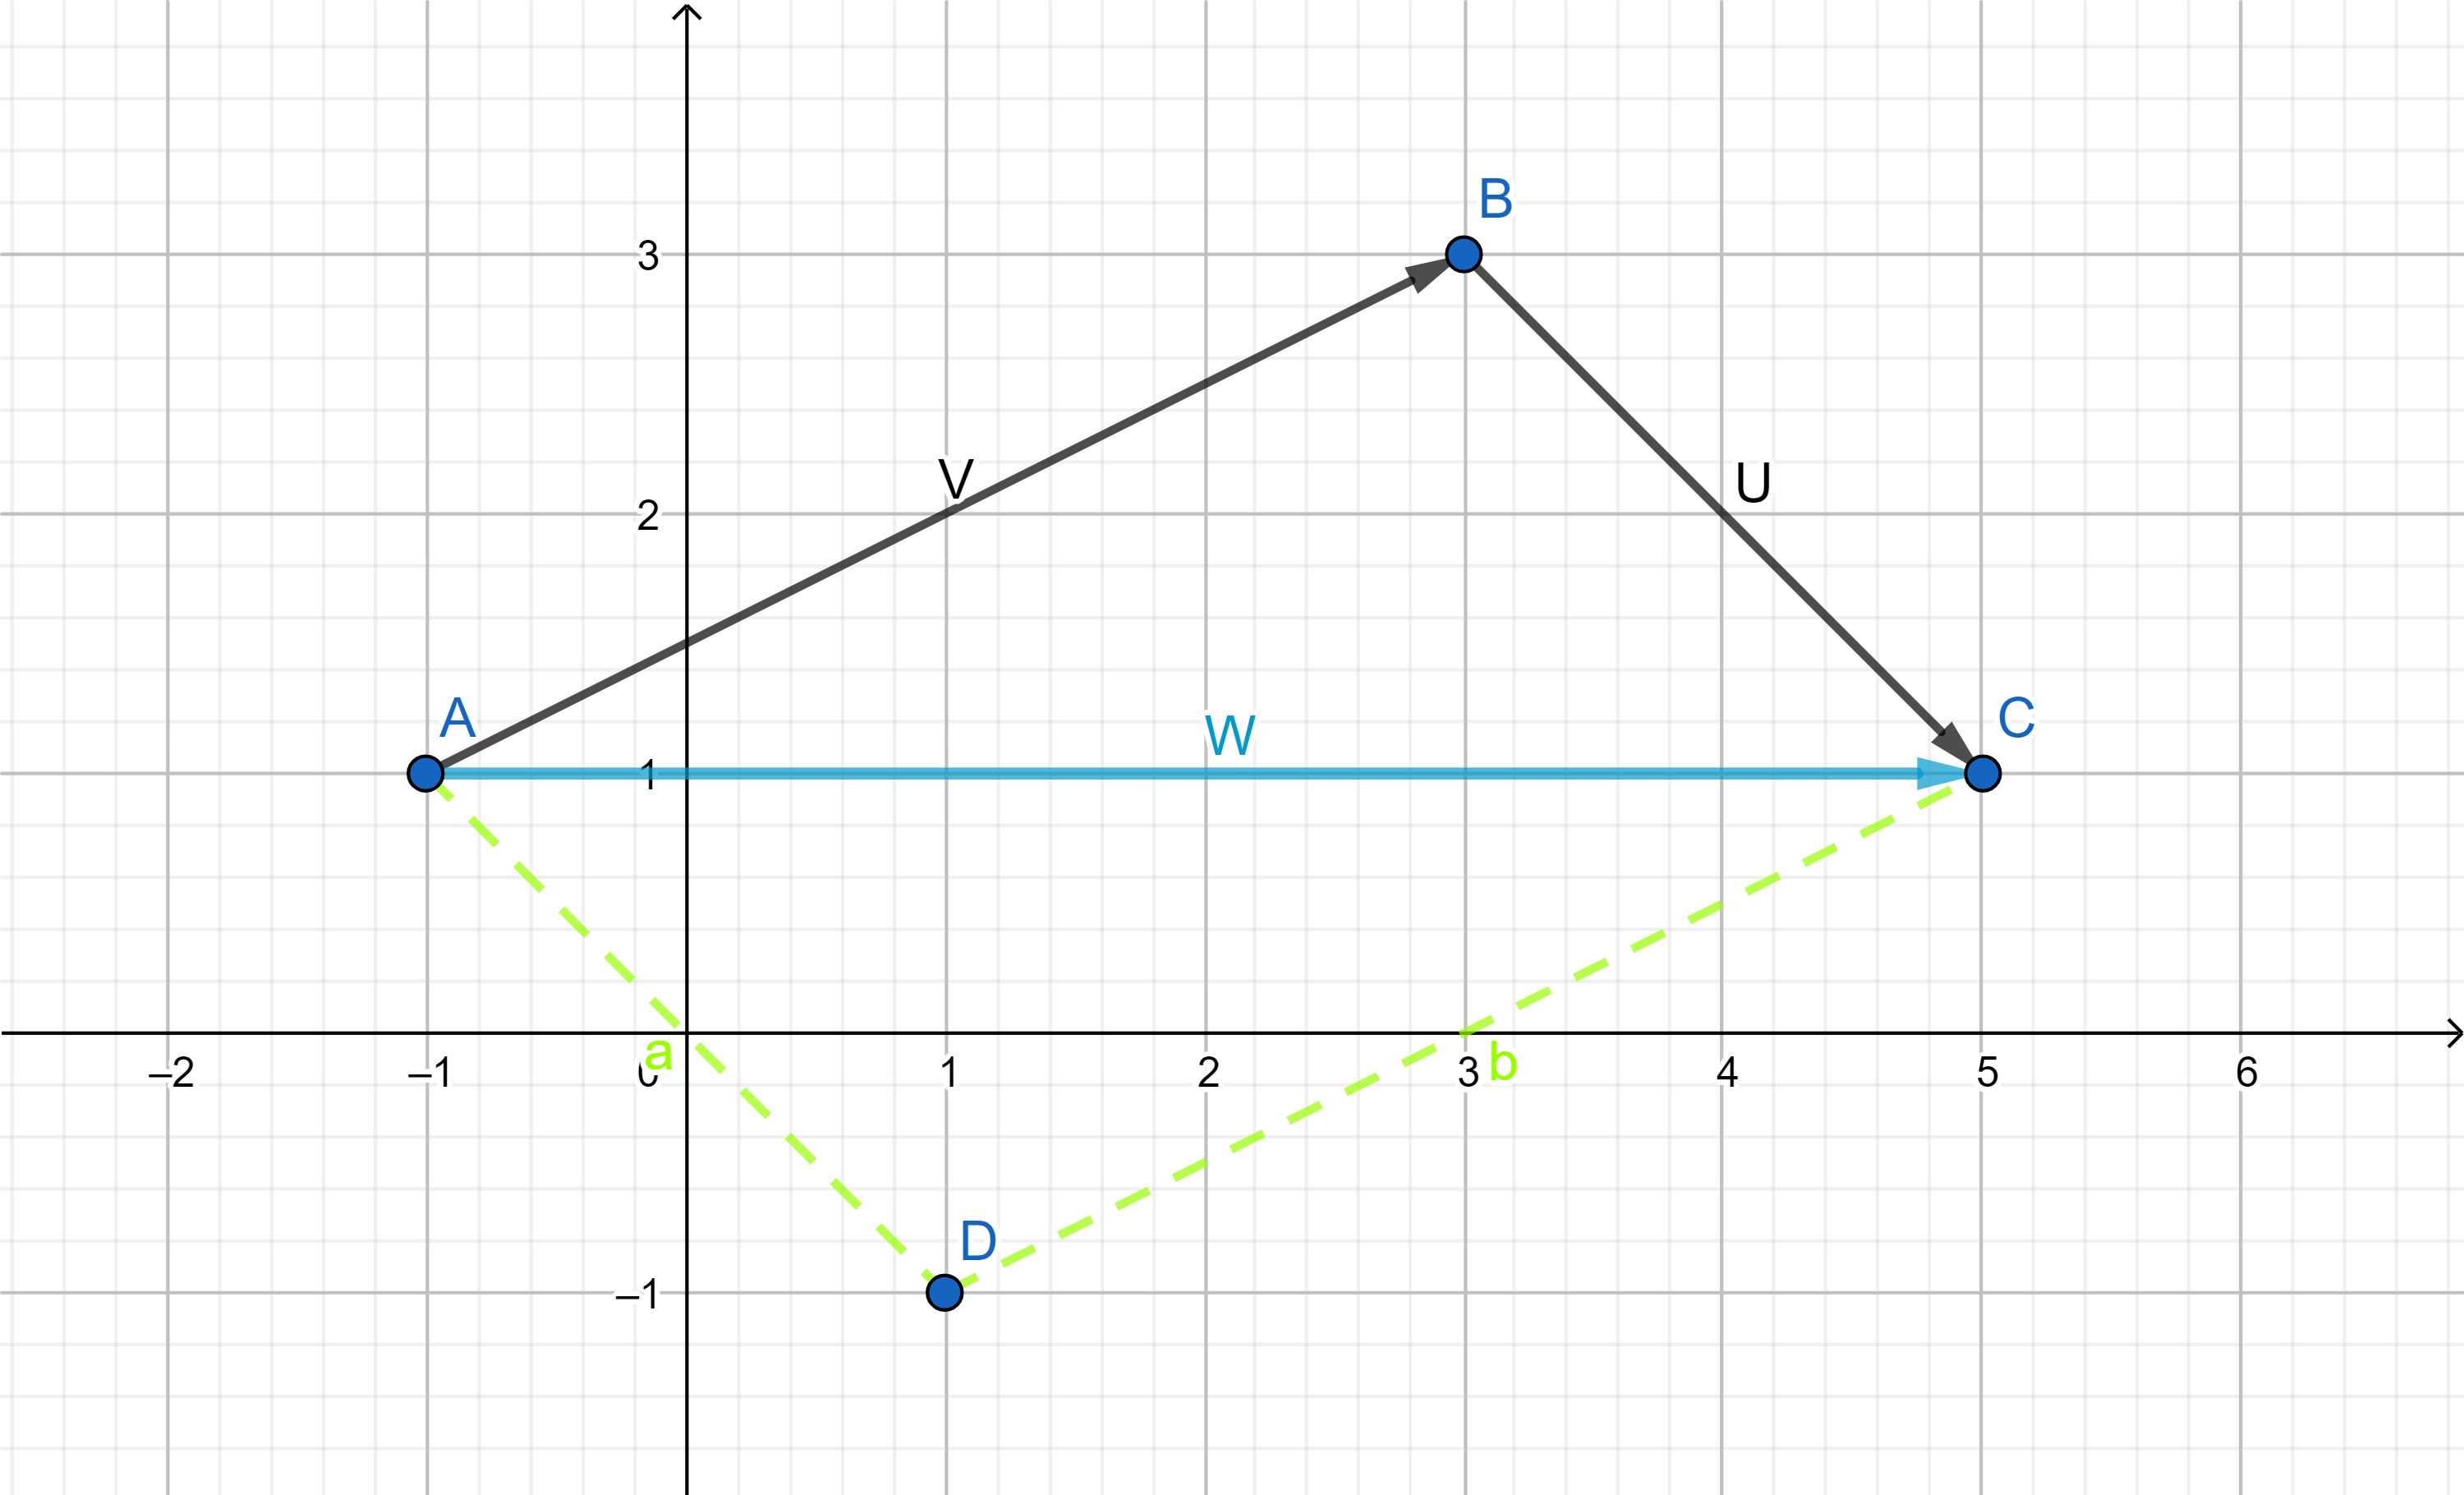
\includegraphics[width=0.60\textwidth]{Pictures/suma de vectores.png}   
\end{figure}



\begin{figure}
    \centering
    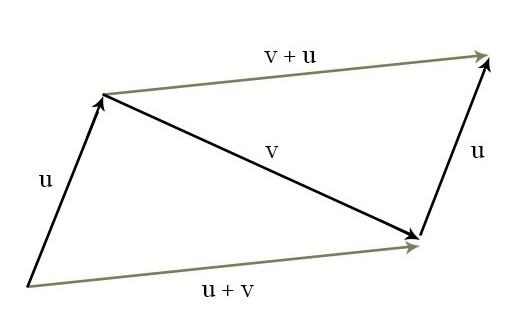
\includegraphics[width=0.50\textwidth]{Pictures/fig.40d.jpg}
   \caption{$~\vec{u}~ + ~\vec{v}~ = ~\vec{v}~ + ~\vec{u}~$}
    \label{fig:suma}
\end{figure}

\bigskip


\bigskip

\bigskip

\begin{remark} 
%$\\$
%\vspace{1.5cm}
\begin{itemize}

\item 

Los elementos del espacio vectorial reciben el nombre genérico de \textit{vectores}.
\item 
Las primeras cuatro propiedades se refieren a la suma en $V$, las dos que siguen a la multiplicación de elementos de $V$  por escalares y las dos últimas son las propiedades distributivas de una operación con respecto a la otra.
\item 
Si K es $\mathbb{R}$ se dice que $V$ es \textit{un espacio vectorial real}, y si K es  $\mathbb{C}$ se dice que es \textit{un espacio vectorial complejo}.
\end{itemize}
%\hfill$\blacktriangle$
\end{remark}

%\begin{enumerate}[label=\itembolasazules{\arabic*}]

\begin{example}
$\mathbb{R}$ es un espacio vectorial sobre $\mathbb{Q}$, $\mathbb{C}$ es un espacio vectorial sobre $\mathbb{R}$ y  sobre $\mathbb{Q}$.
$\mathbb{R}^{2}$ o $\mathbb{R}^{3}$ (vectores en el plano, o en el espacio), con las operaciones usuales son espacios vectoriales sobre $\mathbb{R}$.
\end{example}

\bigskip

\begin{example}   
$$K^n=\{(x_1,x_2, \cdots, x_n), ~ x_j \in K, j=1,2, \cdots, n\}$$
con las operaciones usuales es un espacio vectorial sobre K. En particular, $\mathbb{R}^{n}$ es un espacio vectorial real y  $\mathbb{C}^{n}$ es un espacio vectorial complejo.
\end{example}

\bigskip

\begin{example}
Sea $P_K \left[x\right]$ el conjunto de todos los polinomios en la variable $x$ sobre el cuerpo $K$, es decir, todos los elementos de la forma
$$p(x)= a_0 + a_1 x +a_2 x^2 + \cdots + a_n x^n  + \cdots $$ 
donde los coeficientes $a_j \in K$ con las operaciones suma de polinomios y multiplicación por escalares.  $P_K\left[x\right]$ es un espacio vectorial sobre $K$.
\end{example}

\bigskip


\begin{example} 
Sea $C(\left[a,b\right])$ el conjunto de todas las funciones continuas definidas en el intervalo real $[a,b]$, con valores en $\mathbb{R}$, $\left \{ f: [a,b]  \rightarrow  \mathbb{R} \right \}$ con las operaciones suma de funciones,

$$(f+g)(x)=f(x)+g(x),$$ y multiplicación de una función por un escalar,
$$(af)(x)=a(f(x)).$$
Puede comprobarse fácilmente  que  $C([a,b])$ es un espacio vectorial. El elemento neutro es la función nula.
\end{example}


\bigskip


\begin{example} 
El conjunto $S(A)$ de soluciones del sistema homogéneo $A\vec{X}=\vec{0}$, donde $A \in \mathbb{R}^{m \times n}$ y $\vec{X}=(x_1, x_2, \cdots, x_n)$ $\in \mathbb{R}^{n}$ es un  espacio vectorial sobre $\mathbb{R}$. Es un subespacio de  $\mathbb{R}^{n}$.
\end{example}

\bigskip

\begin{remark}
Los siguientes son algunos resultados que se deducen de las propiedades que definen un espacio vectorial y se dejan como ejercicio para el lector.

\begin{itemize}
\item[$\bullet$]  El elemento neutro de un espacio vectorial es único. 

\item[$\bullet$]  El opuesto de cada elemento en un espacio vectorial es único. 

\item[$\bullet$]   Para todo $\vec{u}$ de un espacio vectorial $V$, $0.\vec{u}=\vec{0}$. 


\item[$\bullet$] Para todo elemento $\vec{u}$ de un espacio vectorial $V$, $(-1)\vec{u}$ es su opuesto.

\item[$\bullet$] En todo espacio vectorial $V$, $a$ $\vec{0}=\vec{0}$, donde $a\in $K y $\vec{0}$ es el elemento neutro de $V$.

\end{itemize}
\end{remark}


\section{Subespacio vectorial}
\label{Subespacio vectorial}
Algunos subconjuntos de un espacio vectorial $V$ son a su vez espacios vectoriales con las operaciones definidas en $V$; estos subconjuntos especiales reciben el nombre de \textit{subespacios vectoriales} de $V$.

\bigskip

\begin{definition}\index{Subespacio vectorial}
Un \textit{subespacio vectorial} de un espacio vectorial $V$ es un subconjunto $S$ no vacío  de $V$, que a su vez es un espacio vectorial con las operaciones definidas en $V$.
\end{definition}


\bigskip

\begin{remark}
Para demostrar que un subconjunto  $S$ es un subespacio vectorial no es necesario comprobar de nuevo que satisface todas las propiedades del espacio vectorial. Es suficiente demostrar que  contiene al vector nulo, que la suma de dos elementos de $S$ es otro elemento de $S$, y que la multiplicación de un elemento de $S$ por un elemento del cuerpo K, es otro elemento de $S$:


\bigskip

 
\begin{enumerate}
\item  $\vec{0} \in S$
\item Si $\vec{u}$ y $\vec{v}$ $ \in$ $S$, $~\vec{u}~+  ~\vec{v}~$ $ \in$ $S$

\item Si $a$ $ \in$ $K$ y $\vec{u}$ $ \in$ $S$, $a~\vec{u}~$ $\in$ $S$

\end{enumerate}
%\hfill$\blacktriangle$
\end{remark}


\begin{figure}
    \centering
    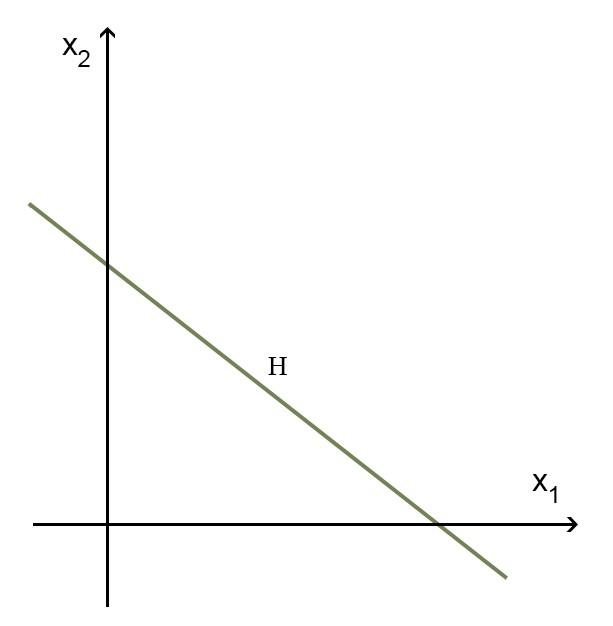
\includegraphics[width=0.40\textwidth]{Pictures/fig.41.jpg}
   \caption{Recta que no pasa por el origen. }
    \label{rectanon}
\end{figure}
%\begin{center}
 %\begin{tikzpicture}[scale=1.5]
 %\label{rectano}
    % Draw axes
    %\draw [<->,thick] (0,2) node (yaxis) [above] {$x_2$}
      %  |- (3,0) node (xaxis) [right] {$x_1$};
       %     \draw[line width =0.051cm, blue]  (-0.5,1.5) -- (2.5,-0.5);
    %\draw [thick] (1.2,1) node[below]{$H$};
 %\end{tikzpicture}
%\caption{ Figura 2.2. Una recta que no pasa por el origen no es un subespacio vectorial  de $\mathbb{R}^2$.}
%\caption{Una recta que no pasa por el origen no es un subespacio vectorial  de $\mathbb{R}^2$.}
%\end{center}
%\begin{figure}
 %   \centering
    %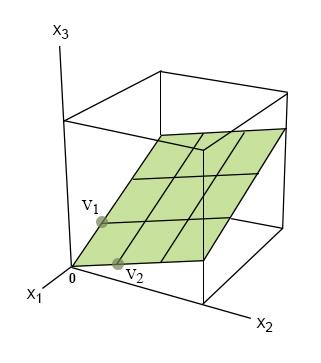
\includegraphics[width=0.50\textwidth]{Pictures/EVfig.2.jpg}
   
    %\label{EVfig. 2}
%\end{figure}
%\begin{example}
%{$S=\{(0,0)\}$ es un subespacio}

%\bigskip


\begin{example}
Sea $V$ un espacio vectorial sobre $K$. $S=\{\vec{0}\}$ es un subespacio de $V$.
\end{example}
\begin{example}
$V$ es un subespacio de $V$.
\end{example}




\begin{example}
Veamos cómo  caracterizar los subespacios de $\mathbb{R}^2$.
\begin{enumerate}
\item
$S=\{(0,0)\}$ es un subespacio.

\item 
Supongamos $S$ un subespacio que contiene algún elemento $\vec{u}$ no nulo. Entonces para todo $a$ $\in R$, $a\vec{u}$ $\in S$. Si esos son todos los elementos de $S$, $S$ es un subespacio y gráficamente es una recta por el origen.

\item 

Si $S$ contiene a un $ \vec{v}$ que no es $a \vec{v}$, contiene a sus múltiplos $a \vec{v}$. 
Luego contiene a dos rectas $L_{\vec{u}}$ y $L_{\vec{v}}$ por el origen. Por la regla del paralelogramo cualquier $\vec{w}$ $\in$ $\mathbb{R}^2$ es suma de un elemento de $L_{\vec{u}}$ y uno de $L_{\vec{v}}$. En consecuencia $S=\mathbb{R}^2$.
\end{enumerate}

\bigskip

Los subespacios de $\mathbb{R}^2$ son entonces, el vector nulo, las rectas por el origen y todo $\mathbb{R}^2$.
\end{example}

\bigskip

\begin{example}
\label{rectanonueva}
Sea $H=\{(x,y) \text{ tales que } y=mx+b \quad m, b \in \mathbb{R}, ~ b \neq 0 \}$ 
(Ver Figura \ref{rectanon}).
$H$ no es un subespacio de $\mathbb{R}^2$. Ya que si $(x_1,y_1)$ y $(x_2,y_2)$  son $2$ puntos sobre la recta $y=mx+b$, $y_1=m x_1+ b$ e $y_2=m x_2+ b$, se tiene que  $y_1+y_2= m(x_1+x_2) + 2 b$,  y entonces, $y_1+y_2  \notin H$.
O bien, directamente,  no es subespacio de $\mathbb{R}^2$ porque $(0,0) \notin H$.
\end{example}
\begin{figure}
    \centering
    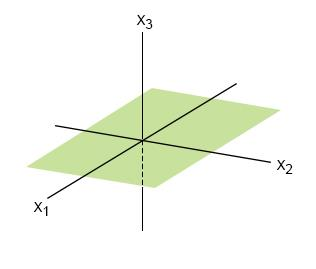
\includegraphics[width=0.60\textwidth]{Pictures/EVfig.1.jpg}
    \caption{El plano $x_1x_2$ es un subespacio de $\mathbb{R}^3$ }
    \label{EVfig.1}
\end{figure}
%\begin{example}
%El  plano por el origen $x_3=0$  (Figura \ref{EVfig.1}) es un subespacio de $\mathbb{R}^3$
%\end{example}
%\vskip1.5cm
\begin{example}
Si $\vec{v}$  $ \in$ $V$, $S=\{a\vec{v}, a\in K \}$ es un subespacio de $V$. Este subespacio se denomina el subespacio generado por $\vec{v}$, y se nota $S=\left\langle \vec{v}\right\rangle$.
\label{ejgenv}
\end{example}

\bigskip
\begin{theorem}
\label{PROP121}
%\begin{thm}
Sean $\vec{v}_1,\vec{v}_2,\cdots,\vec{v}_n$ $ \in$ $V$. Entonces $S=\{a_1 \vec{v}_1+a_2 \vec{v}_2+\cdots +a_n\vec{v}_n, ~ a_i ~ \in K \}$ es un subespacio de $V$. 
\noindent
\begin{proof}

\begin{itemize}
\item
$\vec{0}\in S$ ya que 
$\vec{0} =0 \vec{v}_1+0 \vec{v}_2+\cdots +0\vec{v}_n, ~ 0 ~ \in K $.

\item
Si
 $\vec{u} =a_1 \vec{v}_1+a_2 \vec{v}_2+\cdots +a_n\vec{v}_n, ~ a_i ~ \in K$ y
 
 $\vec{w} =b_1 \vec{v}_1+b_2 \vec{v}_2+\cdots +b_n\vec{v}_n, ~ a_i ~ \in K $,
 entonces
 
 $\vec{u}+\vec{w} =(a_1+b_1) \vec{v}_1+(a_2+b_2) \vec{v}_2+\cdots +(a_n+b_n)\vec{v}_n, 
 
 con (a_i+b_i) ~ \in K $, por lo tanto, $  \vec{u}+\vec{w} \in S$.
 \item
 Si $\alpha \in K$
 $ \alpha \vec{u} = (\alpha a_1) \vec{v}_1+  (\alpha a_2) \vec{v}_2+\cdots + (\alpha a_n)\vec{v}_n, ~ (\alpha a_i) ~ \in K $, por lo tanto $  \alpha \vec{u}  \in S$
 \end{itemize}
 Se tiene, entonces, que $S$ es un subespacio de $V$.
 \end{proof}
%\end{thm}
\end{theorem}





\begin{remark}
El espacio vectorial $\mathbb{R}^2$ no es un subespacio de $\mathbb{R}^3$. $\mathbb{R}^2$ ni siquiera es un subconjunto  de $\mathbb{R}^3$.  En cambio el conjunto


$$S=\left \{ \left( \begin{array}{c} x_1 \\ x_2 \\ 0\end{array}\right) \quad x_1,~x_2 \in \mathbb{R}   \right\}$$

\bigskip
\noindent
sí es un subconjunto y un subespacio de $\mathbb{R}^3$ (Ver Figura \ref{EVfig.1}).
%\hfill$\blacktriangle$
\end{remark}


\begin{example}
 $P_\mathbb{R}^{(n)}\left[t\right]$ (polinomios en $t$  de grado $\leq n$, con coeficientes reales) es un subespacio vectorial de $P_\mathbb{R}\left[t\right]$; a su vez, $P_\mathbb{R}\left[t\right]$ es un subespacio vectorial  del espacio vectorial de las funciones continuas en $\mathbb{R}$.
\end{example}
% figuras subespacios

\begin{figure}
    \centering
    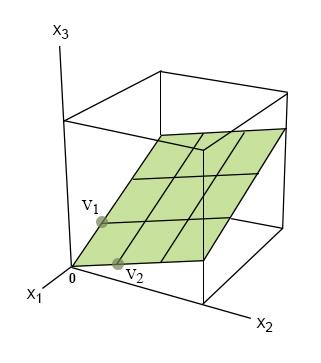
\includegraphics[width=0.50\textwidth]{Pictures/EVfig.2.jpg}
    \caption{Subespacio generado por $\vec{v}_1$ y $\vec{v}_2$ }
    \label{EVfig. 2}
\end{figure}


\begin{example}\index{Combinación lineal}
\label{ejemploLS}
Sea $S=\left\{\vec{u}_1,\vec{u}_2,\cdots,  \vec{u}_n\right\}$ un conjunto de $n$ vectores de un espacio vectorial $V$. Consideremos como en el Ejemplo \ref{ejgenv}  pero con más vectores.
Se define el conjunto de todas las combinaciones lineales de los vectores de $S$, 
$$\bold{L}(S)=\bold{L}(\vec{u}_1,\vec{u}_2,\cdots,  \vec{u}_n)=\left\{\sum_{j=1}^{n}a_j\vec{u}_j,  ~ ~a_j\in K, j=1,2,\cdots,n\right\}$$
El conjunto $\bold{L}(S)$ es un subespacio vectorial de $V$ (ver Proposición \ref{PROP121}), que recibe el nombre de \textsl{subespacio vectorial generado por $S$}. 

En $\mathbb{R}^3$, si $\vec{v}_1$ y $\vec{v}_2$ son dos vectores tales que uno no es múltiplo del otro, entonces,  $\bold{L}(\vec{v}_1,\vec{v}_2,  )$ es un plano que pasa por el origen.  Es un subespacio de $\mathbb{R}^3$; se muestra en la  Figura \ref{EVfig. 2}.




\end{example}

%\vskip1.5cm

\begin{example}
\label{ejintsub}
Sean $a_1, a_2, \cdots, a_n \in K $ fijos.  

$S=\{ (x_1,x_2,\cdots, x_n) \in K^n, a_1x_1+a_2x_2+\cdots +a_nx_n=0\}$ es un subespacio de $K^n$.
\end{example}
%figura Nul A


\begin{example}\index{Espacio nulo de una matriz}
\label{ejsistema}
Dada una matriz $A \in \mathbb{R}^{m \times n}$ , y de rango $r$, todas las soluciones del sistema de ecuaciones homogéneo
$$A\vec{X}=\vec{0}, \qquad  \vec{X}\in \mathbb{R}^n$$
constituyen un subespacio vectorial de $\mathbb{R}^n$, conocido como \textit{espacio nulo} de la matriz $A$. Se anota $Nul(A)$  y se muestra en la  Figura \ref{EVfig. 3.}.


\bigskip

Para el sistema homogéneo:
\begin{equation} 
\left\{ \begin{array} {ccl} \nonumber
                    2y-z+w &\ =&0      \\
                     3x+y+10z+5w &\ = &0  \\
                    x+3z + w &\ =&0 \label{ejemplosist}
                   \end{array}
           \right.
\end{equation}

\bigskip
\noindent
luego de realizar operaciones elementales sobre las filas de la matriz de coeficientes del sistema (método de eliminación gaussiana), se llega a la matriz escalonada:

\[ \left( \begin{array}{cccc}
3 & 1 & 10 & 5\\0 & 2 & -1 &1  \\ 0 & 0 & -1/2 & 1/2 
\end{array}
\right )
\]

\bigskip

\noindent
de donde la solución es $z=-w$, $y=-w$ y $x=2w$. El subespacio  de soluciones del sistema homogéneo es, entonces,

$$S=Nul(A) = \langle (2,-1,-1,1) \rangle $$
\end{example}
%\end{enumerate}


\begin{figure}
    \centering
    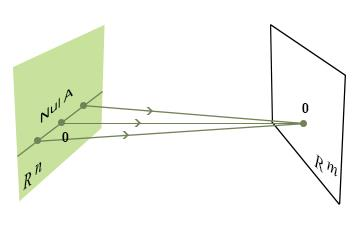
\includegraphics[width=0.60\textwidth]{Pictures/EVfig.3.jpg}
    \caption{Espacio nulo de una matriz $A$.}
    \label{EVfig. 3.}
\end{figure}

\begin{remark}
\label{SHSNH}
Así como vimos que las rectas que no pasan por el origen no son un subespacio de $\mathbb{R}^2$ (Ejemplo  \ref{rectanonueva}), las soluciones de un sistema no homogéneo 
$$A\vec{X}=\vec{b}, \qquad  \vec{b} \neq \vec{0}$$  son un subconjunto pero no un subespacio de    $\mathbb{R}^n$.
%\hfill$\blacktriangle$
\end{remark}

\bigskip

\index{Hamilton, William R.}
\begin{parchment}[William Rowan Hamilton (1805 - 1865)]{ Fue un matemático británico. Fue uno de los fundadores de la escuela británica moderna de matemáticas puras e hizo importantes contribuciones al desarrollo de la óptica, la dinámica, y el álgebra. Su descubrimiento del cuaternión, junto con su sistematización de la dinámica, son sus trabajos más conocidos. Este último trabajo sería decisivo en el desarrollo de la mecánica cuántica, donde un concepto fundamental llamado hamiltoniano lleva su nombre.
Hamilton fue el cuarto de los nueve hijos. Vivían en Dublín. Se dice que Hamilton demostró un inmenso talento a una edad muy temprana. 
Su tío observó que Hamilton, había mostrado una asombrosa habilidad para aprender idiomas. A la edad de siete años, ya había hecho un progreso considerable con el hebreo, y antes de los trece años, bajo la supervisión de su tío (un lingüista), había adquirido conocimientos casi en tantos idiomas como años de edad tenía (idiomas europeos clásicos y modernos, y persa, árabe, hindustaní, sánscrito e incluso maratí y malayo).
Hamilton es reconocido como uno de los científicos más destacados de Irlanda, y a medida que la nación se vuelve más consciente de su herencia científica, cada vez se lo celebra más. Se dice que se le permitía pisar el césped de la Universidad, algo totalmente prohibido. Este hecho camina entre la realidad y la ficción. Posiblemente ocurriera que, absorto en sus meditaciones, descuidara esta prohibición y accidentalmente caminase por los jardines. Esta anécdota seguramente sirve para dar idea de la categoría de Hamilton como uno de los grandes matemáticos de su tiempo y de la historia.
El Instituto Hamilton está dedicado a la investigación sobre matemáticas aplicadas en la Universidad Maynooth. 
Irlanda emitió dos sellos conmemorativos en 1943 para celebrar el centenario del anuncio de los cuaterniones. El Banco Central de Irlanda acuñó en 2005 una moneda de plata conmemorativa de 10 euros para conmemorar los 200 años desde su nacimiento.
Los talleres de mantenimiento más nuevos del sistema de tranvías de Dublín (LUAS), llevan su nombre.

En su juventud, Hamilton tuvo un telescopio y se convirtió en un experto en el cálculo de fenómenos celestes, como por ejemplo, la determinación de la visibilidad de los eclipses de luna. Fue elegido Astrónomo Real de Irlanda y se instaló en el Observatorio de Dunsink, donde permaneció hasta su muerte en 1865.
Hoy en día, Hamilton no es reconocido como un gran astrónomo, aunque durante su vida si gozó de esta consideración. Sus conferencias de introducción a la astronomía fueron famosas; además de sus alumnos, atrajeron a muchos eruditos y poetas, e incluso a damas; en aquellos días una hazaña notable. La poetisa Felicia Hemans escribió su poema "La oración del estudiante solitario" después de escuchar una de sus conferencias.  \cite{hamilton}}
\end{parchment}

\bigskip

\section{Base y dimensión de un espacio vectorial}\index{Independencia lineal}\index{Sistema de generadores}

Sea $V$ un espacio vectorial sobre un cuerpo K; un número finito de vectores  $\vec{v}_1, \vec{v}_2, ,\cdots, \vec{v}_n$  se dice que son \textit{linealmente dependientes} si existen $n$ elementos de K, $a_1, a_2, ,\cdots, a_n$  no todos nulos, tal que 
$$a_1\vec{v}_1+a_2\vec{v}_2+\cdots +a_n\vec{v}_n=\vec{0}$$

Si los vectores $\vec{v}_1, \vec{v}_2, ,\cdots, \vec{v}_n$ no son linealmente dependientes, se dice que son \textit{linealmente independientes}; por lo tanto los vectores $\vec{v}_1, \vec{v}_2, ,\cdots, \vec{v}_n$  son linealmente independientes si cualquier igualdad como la anterior implica que todos los elementos de K, $a_1, a_2, ,\cdots, a_n$  son  nulos.

Si en la igualdad anterior $a_n$ es no nulo, podemos escribir
$$\vec{v}_n=- \frac{ a_1}{a_n}\vec{v}_1- \frac{ a_1}{a_n}\vec{v}_2+\cdots - \frac{ a_{n-1}}{a_n}\vec{v}_{n-1}$$
 y decimos que $\vec{v}_n$ es una \textit{combinación lineal} de los vectores $\vec{v}_1, \vec{v}_2, ,\cdots$, $\vec{v}_{n-1}$. En general, se dice que $\vec{v}$ es combinación lineal de los vectores $\vec{v}_1, \vec{v}_2, \cdots, \vec{v}_k$, si existen  $a_1, a_2, ,\cdots, a_k ~ \in K$  tal que 
$$\vec{v}=a_1\vec{v}_1+a_2\vec{v}_2+\cdots +a_k\vec{v}_k$$

\bigskip

Un conjunto finito de vectores $\{ \vec{v}_1,\vec{v}_2,\cdots, \vec{v}_k\}$ de un espacio vectorial $V$ se dice que es \textsl{un sistema de generadores} de $V$ si todo elemento de $V$ se puede escribir como una combinación lineal de los vectores $\vec{v}_1,\vec{v}_2,\cdots$, $\vec{v}_k$.

\bigskip

\bigskip



\begin{theorem}
    Un conjunto finito de vectores linealmente indepen-\ dientes de un espacio vectorial $V$ no puede contener un subconjunto de vectores que sean linealmente dependientes. 
\begin{proof}
    

Si $\{ \vec{v}_1,\vec{v}_2,\cdots, \vec{v}_n\}$ son linealmente independientes y suponemos que $\{ \vec{v}_1,\vec{v}_2,\cdots, \vec{v}_k\}$, $k\leq n$ son linealmente dependientes se tendría 
$$\vec{v}=a_1\vec{v}_1+a_2\vec{v}_2+\cdots +a_k\vec{v}_k=\vec{0}$$
con no todos los $a_j$ nulos; basta observar que, entonces,


$$a_1\vec{v}_1+a_2\vec{v}_2+\cdots +a_k\vec{v}_k+0\vec{v}_{k+1}+ \cdots + 0\vec{v}_n=\vec{0}$$
con lo cual los originales serían linealmente dependientes.
\end{proof}
\end{theorem} 

\bigskip

Antes de exponer algunos ejemplos es conveniente realizar algunas observaciones.
\begin{remark}

\begin{itemize}

\item 
%\bigskip

Todo conjunto finito de vectores que contiene al elemento neutro (o nulo) es linealmente dependiente; basta observar que 

$$a \vec{0}+0\vec{v_2}+\cdots +0\vec{v_n}=\vec{0}$$
para cualquier $a\in K $.


%\bigskip



\item 
Tres vectores no nulos de $\mathbb{R}^2$ son siempre linealmente dependientes.



\item 
En general, $n+1$  vectores  de $K^n$ son siempre linealmente dependientes.

\end{itemize}
%\hfill$\blacktriangle$
\end{remark}
\bigskip



\bigskip


\begin{example}\index{Espacio fila de una matriz}
\label{ejuis}
Si $\vec{u}_1=(1,0,1)$, $\vec{u}_2=(-1,1,0)$ y $\vec{u}_3=(1,1,2)$,  $\bold{L}(\vec{u}_1,\vec{u}_2,  \vec{u}_3)$ es un subespacio vectorial de $\mathbb{R}^3$. No es todo $\mathbb{R}^3$ porque  estos vectores no son linealmente independientes, ya que,  se anula el determinante de la matriz que tiene esos vectores  como filas:
\[ \left| \begin{array}{ccc}
1 &0 &1\\-1 &1 & 0 \\1&1&2
\end{array}
\right |=0
\]

Para hallar el subespacio que generan  esos vectores se realizan operaciones elementales sobre las filas, y se llega a la matriz escalonada:


\[ \left( \begin{array}{ccc}
1 &0 &1\\0 &1 & 1 \\0 &0 &0 
\end{array}
\right)
\]

\bigskip

La última fila de ceros indica que el vector $\vec{u}_3$ es combinación lineal de $\vec{u}_1$ y $\vec{u}_2$.
Entonces los vectores generados por $\vec{u}_1,~\vec{u}_2$ y  $\vec{u}_3$ son de la forma $\alpha (1,0,1)+ \beta (0,1,1)= ( \alpha, \beta, \alpha + \beta) $ por lo que 
$\bold{L}(\vec{u}_1,\vec{u}_2,  \vec{u}_3)$ es el plano por el origen  $z=x+y$.
Considerando la matriz que tiene los vectores $\vec{u}_i$ como filas, $\bold{L}(S)$ es el espacio generado por las filas de la matriz, conocido como \textit{espacio fila}.
\end{example}

\begin{example}
\label{ejpk}
Las funciones $p_0(t)=1$, $p_1(t)=t$, $p_2(t)=t^2$, $\cdots$, $p_n(t)=t^n$, son linealmente independientes, ya que si tenemos la igualdad

$$a_01+a_1t+a_2t^2  + \cdots + a_nt^n=0$$
para todo $t\in \mathbb{R}$, resultan $a_0=a_1=a_2=\cdots a_n=0$.

Para demostrarlo basta tomar $n$ puntos $t_i$ distintos y resolver el sistema. Tiene como única solución la trivial. El determinante del sistema es conocido como determinante de Vandermonde.
\end{example}




\begin{example}

Las funciones $f(t)=cos^2(t)$,  $g(t)=sen^2(t)$ y $h(t)=1$ son linealmente dependientes en $C(\left[0,2\pi\right])$ ya que $cos^2(t) +sen^2(t)=1$, y entonces es posible escribir al vector nulo con coeficientes no todos nulos $$1 cos^2(t) +1 sen^2(t)+ (-1)1 =0.$$

Por otro lado, ejemplos de funciones linealmente independientes son $f_1(t)= e^{k_1 t}$ y $f_2(t)= e^{k_2 t}$ con $k_1 \neq k_2$.
\end{example}

\begin{remark}
La independencia lineal de funciones  es de importancia para describir el conjunto solución de ecuaciones diferenciales y se determina a partir del cálculo de un determinante conocido como Wronskiano  (ver \cite{grossman}).
%\hfill$\blacktriangle$
\end{remark}


\begin{example}
$S=\{ cos(nx),sen(mx)\}_{n,m \in \mathbb{N}}$  es un conjunto de funciones linealmente independiente en $C(\left[0,2\pi\right])$.
\end{example}

\begin{remark}
Al desarrollo en serie de una función en   términos de las funciones $cos(nx)$ y $sen(mx)$ con $n,m \in \mathbb{N}$ se lo conoce como Serie de Fourier.
%\hfill$\blacktriangle$
\end{remark}


\bigskip
%\vskip1.5cm
\begin{definition}\index{Base de un espacio vectorial}
\label{base}
Un conjunto finito de vectores $\{ \vec{e}_1,\vec{e}_2,\cdots, \vec{e}_n\}$ se dice que es una \textit{base} de un espacio vectorial $V$ si se cumplen las dos condiciones siguientes:
\begin{enumerate}

\item
Los vectores $ \vec{e}_1,\vec{e}_2,\cdots, \vec{e}_n$ son linealmente independientes.
\item
Todo elemento de $V$ es una combinación lineal de los vectores $ \vec{e}_1,\vec{e}_2,\cdots, \vec{e}_n$.

\end{enumerate}

\end{definition}
%\textbf{DEFINICIÓN:}

\bigskip

\begin{remark}

La segunda condición de esta definición es equivalente al hecho de que el conjunto de vectores $\{\vec{e}_1,\vec{e}_2,\cdots, \vec{e}_n \}$ sea un sistema de generadores de $V$. Sin embargo, no todo sistema de generadores de un espacio vectorial $V$ es una base. Se deja al lector pensar ejemplos.
%\hfill$\blacktriangle$
\end{remark}




\bigskip


\begin{example}\index{Base canónica}


Si $\vec{e}_j=(0,0,\cdots,1,\cdots,0)\in K^{n}$, donde $1$ ocupa el lugar $j$, se tiene que $\vec{e}_1,\vec{e}_2,\cdots, \vec{e}_n$ son linealmente independientes y además si $\vec{x}=(x_1,x_2, \cdots,x_n)\in K^{n}$, se tiene que 
$$\vec{x}=\sum_{j=1}^{n}x_j\vec{e}_j$$

Por lo tanto $\left\{\vec{e}_1,\vec{e}_2,\cdots, \vec{e}_n\right\}$ es una base de $K^{n}$, que recibe el nombre de \textit{base canónica} de este espacio.  En la Figura \ref{EVfig. 4} se muestra  para el caso $n=3$.

\bigskip
\end{example}
\begin{figure}
    \centering
    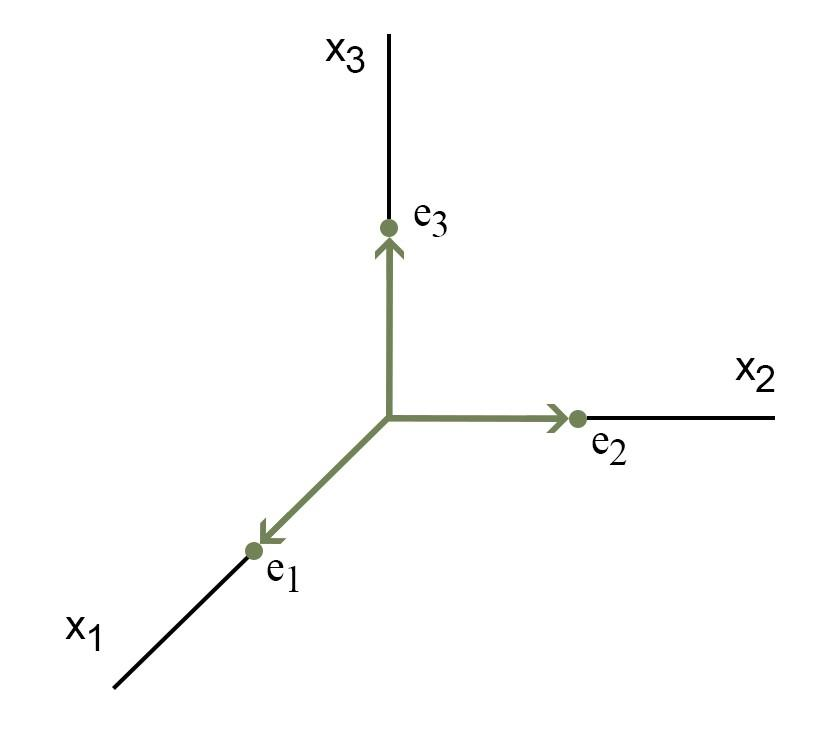
\includegraphics[width=0.50\textwidth]{Pictures/EVfig.4.jpg}
    \caption{Base canónica  de $\mathbb{R}^3$. }
    \label{EVfig. 4}
\end{figure}



\begin{example}
Dada una matriz $A$ de $m$ filas y $n$ columnas, y de rango $r$, todas las soluciones del sistema de ecuaciones homogéneo
$$A \vec{X}=\vec{0}, \qquad   \vec{X} \in \mathbb{R}^n$$
constituyen un subespacio vectorial de $\mathbb{R}^n$ generado por  $n-r$ vectores. Recordar que $r$ es la cantidad de pivotes al realizar operaciones elementales sobre las filas de la matriz  en eliminación gaussiana.

\bigskip
En el Ejemplo \ref{ejsistema} se tiene que  $m=3$, $n=4$ y el rango $r=3$. $S=Nul(A) = \langle (2,-1,-1,1) \rangle $,  es un subespacio de dimensión 
$n-r=4-3=1.$
\end{example}
\bigskip

\begin{example}

El conjunto $\left\{1,t,\cdots, t^{n}\right\}$ es una base de $P_K^{(n)}\left[t\right]$, ya que son polinomios linealmente independientes de acuerdo con el resultado del Ejemplo \ref{ejpk} (para $K= \mathbb{R}$), y todo polinomio $p$ de grado inferior o igual a $n$ puede escribirse de la forma
$$p(t)=a_01+a_1t+a_2t^{2} + \cdots +a_nt^{n}$$

 Para   para el caso $n=2$ se tiene la base $\left\{1,t, t^{2}\right\}$ que se muestra  en la Figura \ref{EVfig5}.
\end{example}
% figura base de P2

\begin{figure}
    \centering
    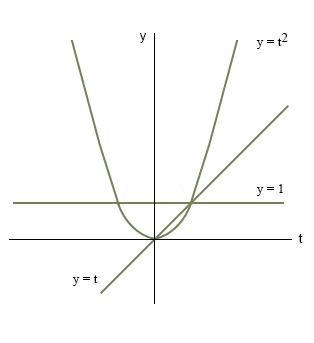
\includegraphics[width=0.50\textwidth]{Pictures/EVfig.5.jpg}
    \caption{Base canónica de $P_R^{(2)}\left[t\right]$ }
    \label{EVfig5}
\end{figure}

\bigskip

\begin{remark}
    El conjunto $\left\{1,t,\cdots, t^{n}\right\}$ no es una base de $P_K\left[t\right]$, ya que el polinomio $p(t)=t^{n+1}$ no es combinación lineal de estos. Se puede ver que ningún conjunto finito de polinomios  genera a $P_K\left[t\right]$ (ver  \cite{grossman}) .
%\hfill$\blacktriangle$
\end{remark}

\bigskip

\newpage

%\vskip0.5cm
\textbf{Coordenadas de un vector}\index{Coordenadas}

Si $\left\{\vec{e}_1,\vec{e}_2,\cdots, \vec{e}_n\right\}$ es una base de un espacio vectorial $V$ y $\vec{v}$ es cualquier elemento de $V$ podemos escribir a $\vec{v}$ como combinación lineal de $\vec{e}_1,\vec{e}_2,\cdots, \vec{e}_n$, de la forma

$$\vec{v}=  a_1\vec{e}_1+a_2\vec{e}_2+\cdots +a_n \vec{e}_n$$
con $a_j \in K$. Los números $a_1,a_2,\cdots,a_n$ se denominan \textit{coordenadas} de $\vec{v}$ con respecto a la base $\vec{e}_1,\vec{e}_2,\cdots, \vec{e}_n$.

\bigskip

\bigskip

\bigskip


\begin{theorem}
    
Las coordenadas de un vector $\vec{v}$ con respecto a una base son únicas.
 \begin{proof}
     Si suponemos se tienen  coordenadas $a_i$ y $b_i$, ~$i=1, \cdots n$ para un mismo vector $\vec{v}$,

$$\vec{v}=  a_1\vec{e}_1+a_2\vec{e}_2+\cdots +a_n \vec{e}_n$$
y 
$$\vec{v}=  b_1\vec{e}_1+b_2\vec{e}_2+\cdots +b_n \vec{e}_n$$
\noindent
se tiene  que 
$$\vec{0}=  (b_1-a_1)\vec{e}_1+(b_2-a_2)\vec{e}_2+\cdots +(b_n-a_n) \vec{e}_n$$
Como  $\vec{e}_1,\vec{e}_2,\cdots, \vec{e}_n$ son linealmente independientes,  $b_1=a_1$,  $b_2=a_2$, $\cdots$, $b_n=a_n$.
\end{proof}
\end{theorem}
%\vskip0.25cm

\bigskip



%\vskip1.5cm

\begin{example}


Sea $V=\mathbb{R}^{3}$    y sea $E$  la base canónica. Las coordenadas de un vector $\Vec{v}$ se anotan  $(x,y,z)_E=(x,y,z)$.


Si en lugar de la base canónica la base es $B=\left\{(1,1,1),(1,1,0),(1,0,0) \right\}$,  las coordenadas  de  un vector $(x,y,z)$  son $(z,y-z,x-y)_B$ y se escribe la igualdad $(x,y,z)=(z,y-z,x-y)_B$.

Esto se obtiene escribiendo  $(x,y,z)$ como combinación lineal de los vectores de $B$, $$(x,y,z)=a(1,1,1)+b(1,1,0)+c(1,0,0),$$ y  resolviendo el sistema lineal:

\begin{equation} 
\left\{ \begin{array} {ccl} \nonumber
                    a + b + c &\ =&x     \\
                     a + b + 0c &\ = &y  \\
                    a +0b +0c  &\ =&z \label{ejemplosist}
                   \end{array}
           \right.
\end{equation}


\end{example}

%coordenadas  ver ejemplos de la pag 22 


\bigskip

Un mismo espacio vectorial puede poseer varias bases; nuestro próximo objetivo es demostrar que todas ellas han de poseer el mismo número de elementos.

\bigskip

\begin{theorem}
\label{Prop1}
Si $V$ es un espacio vectorial que posee una base con $\textsl{n}$ elementos, cualesquiera $\textsl{n}+1$ vectores de $V$ son linealmente dependientes.

\bigskip
\begin{proof}


%\noindent
%\textsl{Demostración}

Sea $\left\{\vec{e}_1,\vec{e}_2,\cdots, \vec{e}_n\right\}$ una base de $V$ y sean $\vec{x}_1,\vec{x}_2,\cdots, \vec{x}_n, \vec{x}_{n +1} $,  $n+1$ vectores de $V$,

\bigskip
\noindent
que pueden escribirse como combinación lineal de la base dada:

\bigskip

$\vec{x}_1= \sum_{j=1}^{n} x_{j1}\vec{e}_j,  \qquad \vec{x}_2= \sum_{j=1}^{n} x_{j2}\vec{e}_j,  \qquad \vec{x}_n= \sum_{j=1}^{n} x_{jn}\vec{e}_j,   \qquad $ y $\vec{x}_{n+1}= \sum_{j=1}^{n} x_{jn+1}\vec{e}_j $

\bigskip


Se quiere ver si son linealmente independientes.  Nos preguntamos  si existen $a_i$ no todos nulos tales que 
  
  \bigskip
  
 $a_1\vec{x}_1+a_2\vec{x}_2+\cdots + a_n \vec{x}_n + a_{n+1}\vec{x}_{n +1} = \vec{0} $  
 
 \bigskip
 
Reemplazando, se  tiene

 \bigskip
 
 $   a_1  (\sum_{j=1}^{n} x_{j1}\vec{e}_j)  +  a_2  (\sum_{j=1}^{n} x_{j2}\vec{e}_j) +  a_n  (\sum_{j=1}^{n} x_{jn}\vec{e}_j) \\ + a_{n+1}  (\sum_{j=1}^{n} x_{j n+1}\vec{e}_j)= \vec{0}    $
 
  \bigskip
  
  Al desarrollar las sumas anteriores y  reordenar  sacando factor común los vectores $\vec{e}_j$,  se obtiene
  
  \bigskip
  
  
  $\vec{e}_1 ( x_{11}a_1+x_{12}a_2+ \cdots +x_{1n}a_n   +x_{1n+1}a_{n +1})=0  $
  
  \bigskip
  
  $\vec{e}_2 ( x_{21}a_1+x_{22}a_2+\cdots +x_{2n}a_n   +x_{2n+1}a_{n +1})=0  $
  
  \bigskip
  
  $\cdots$
  
   \bigskip
  
  $\vec{e}_n ( x_{n1}a_1+x_{n2}a_2+\cdots  +x_{nn}a_n   +x_{nn+1}a_{n +1})=0  $
  
  \bigskip
  
  Los términos entre paréntesis constituyen  un sistema homogéneo de $n$ ecuaciones con $n+1$ incógnitas, $a_1$, $a_2$,   $\cdots$, $a_{n+1}$ por lo que  existe  una solución no trivial ($a_i$ no todos nulos). 
  
  \bigskip
  
  Se concluye, entonces, que  los vectores $\vec{x}_1,\vec{x}_2,\cdots, \vec{x}_n, \vec{x}_{n +1} $ son lineal-\ mente dependientes.
  
  
  
  \end{proof}
\end{theorem} 

\bigskip


%\vskip1.5cm
\begin{remark}
De la proposición anterior se deduce un resultado un poco más general: en un espacio vectorial $V$ que posee una base con $n$ elementos, cualesquiera $m$ vectores de $V$, con $\textsl{m}>\textsl{n}$ son linealmente dependientes. Basta observar que $n+1$ de los $m$ vectores dados han de ser linealmente dependientes, debido a la proposición anterior, y por lo tanto, todos ellos han de formar un conjunto de vectores linealmente dependiente. Este resultado se aplica en la demostración del teorema que sigue.
%\hfill$\blacktriangle$
\end{remark}
%\vskip0.25cm

\bigskip

\bigskip

\bigskip

\index{Fourier, Jean-Baptiste.}
\begin{parchment}
[Jean-Baptiste Joseph Fourier (1768 - 1830)]{ Fue un matemático y físico francés conocido por sus trabajos sobre la descomposición de funciones periódicas en series trigonométricas convergentes llamadas Series de Fourier, método con el cual consiguió resolver la ecuación del calor. La transformada de Fourier recibe su nombre en su honor. Fue el primero en dar una explicación científica al efecto invernadero en un tratado.
Inició sus estudios en la Escuela Superior Benedictina de Auxerre, orientándose inicialmente a la carrera religiosa, hasta que el monarca Luis XV la convirtió en academia militar. Jean-Baptiste fue seleccionado como estudiante en la institución ya reformada, donde permanecería hasta los 14 años de edad, y empezó a ser instruido en idiomas, música, álgebra y matemáticas, materia en la que destacó, lo que le encaminó a dedicarse al estudio de las ciencias.
Posteriormente, participó en la Revolución francesa y, gracias a la caída del poder de Robespierre, se salvó de ser guillotinado. Se incorporó a la Escuela Normal Superior de París en donde tuvo entre sus profesores a los matemáticos Joseph Louis Lagrange y Pierre Simon Laplace. Posteriormente, ocupó una cátedra como docente en la prestigiosa École polytechnique.
Fourier participó en la expedición de Napoleón Bonaparte a Egipto en 1798. 
%Ya designado secretario perpetuo del Instituto de Egipto el 22 de agosto de 1798, presentó numerosas memorias y dirigió una de las comisiones de %exploración del Alto Egipto. Entre las distintas funciones políticas o administrativas que llevó a cabo, destaca la de comisario francés en el Divan. %A la muerte del General en Jefe del Ejército de Oriente Jean Baptiste Kléber a manos de un fanático sirio en su residencia en El Cairo, Fourier, %quien era amigo y colaborador del General Kléber, es designado para pronunciar el elogio fúnebre, el 17 de junio delante del Instituto de Egipto. A %su regreso a Francia en 1801, Napoleón Bonaparte le nombró prefecto de Isère y entre 1802 y 1815, Fourier presentó a Jean-François Champollion a los %veteranos de la expedición de Egipto.
Entró a la Academia de Ciencias Francesa en 1817 y al cabo de cinco años se convirtió en el secretario perpetuo de las secciones de matemáticas y física.
%Murió en París el 16 de mayo de 1830.
Fue en Grenoble donde condujo sus experimentos sobre la propagación del calor que le permitieron modelar la evolución de la temperatura a través de series trigonométricas. Estos trabajos mejoraron el modelado matemático de fenómenos físicos y contribuyeron a los fundamentos de la termodinámica.
Sin embargo, la simplificación excesiva que proponen estas herramientas fue muy debatida, principalmente por sus maestros Laplace y Lagrange.
Publicó en 1822 su Théorie analytique de la chaleur (Teoría analítica del calor), tratado en el cual estableció la ecuación diferencial parcial que gobierna la difusión del calor solucionándola mediante el uso de series infinitas de funciones trigonométricas, lo que establece la representación de cualquier función como series de senos y cosenos, ahora conocidas como las series de Fourier. El trabajo de Fourier provee el impulso para trabajar más tarde en las series trigonométricas y la teoría de las funciones de variables reales.
%Los dos primeros capítulos de la obra citada tratan problemas sobre difusión de calor entre cuerpos disjuntos en cantidad finita. 
Fourier en esta obra dedujo la ecuación en derivadas parciales que rige tal fenómeno, la cual es conocida como la ecuación del calor.  \cite{fourier}}
%En el capítulo III de la obra, titulado Difusión del calor en un cuerpo rectangular infinito Fourier introduce su método original de trabajo con %series trigonométricas.
\end{parchment}


\bigskip

\bigskip


\begin{theorem}
\label{2122}
%\textbf{PROPOSICIÓN 2.1.2.2 :}
Todas las bases de un mismo espacio vectorial $V$ poseen el mismo número de elementos.

\begin{proof}
Sean $\left\{\vec{e}_1,\vec{e}_2,\cdots, \vec{e}_n\right\}$  y $\left\{\vec{e}^{\prime}_1,\vec{ e}^{\prime}_2,\cdots, \vec{e}^{\prime}_m\right\}$ dos bases de un espacio vectorial $V$; por lo anterior $m\leq n$, ya que en caso contrario los vectores de la segunda base serían linealmente dependientes. Similarmente  \\ $n\leq m$
ya que en caso contrario los vectores de la primera base serían linealmente dependientes. Se tiene, por lo tanto, que $n=m$.

\end{proof}
\end{theorem}
%\vskip1.5cm

\bigskip


\index{Dimensión de un espacio vectorial}
El número de elementos que posee una base cualquiera de un espacio vectorial $V$ recibe el nombre de \textit{dimensión} de $V$; este número será designado mediante $dim(V)$. Si el espacio vectorial sólo contiene un elemento, es decir $V=\left\{\vec{0}\right\}$ tiene \textsl{dimensión cero}.

\bigskip


De los ejemplos anteriores podemos deducir los siguientes resultados:

\bigskip

\begin{enumerate}



\item

La dimensión de $K^{n}$  es $n$.
\item

La dimensión  de $P_K^{(n)}\left[t\right]$  es $n+1$.

\item
En el Ejemplo \ref{ejuis}  se puede ver que  $\bold{L}(\vec{u}_1,\vec{u}_2,  \vec{u}_3)$, donde $\vec{u}_1=(1,0,1)$, $\vec{u}_2=(-1,1,0)$ y $\vec{u}_3=(1,1,2)$,  es un subespacio vectorial de $\mathbb{R}^3$ de dimensión $2$ (un plano por el origen).

\end{enumerate}

\bigskip

\bigskip

\begin{remark}\index{Hiperplano}
    En $\mathbb{R}^n$ un \textit{hiperplano} que contiene al vector nulo es un subespacio $H$ de dimensión $n-1$. O sea  
    $$ H=\{ (x_1,x_2, \cdots, x_n): a_1x_1+a_2x_2 +  \cdots a_nx_n=0\}$$
\noindent
    donde $a_1, a_2, \cdots a_n$ son números reales fijos, no todos nulos. Es decir, un hiperplano  generaliza la noción de plano en $\mathbb{R}^3$.
\end{remark}

\bigskip

\begin{remark}
Se llama \textit{nulidad} de una matriz a la dimensión del espacio nulo. \index{Nulidad de una matriz}
\end{remark}
\bigskip

\begin{theorem}
\label{2123}

%\textbf{PROPOSICIÓN  2.1.2.3  :}

Sea $V$ un espacio vectorial de dimensión $n$. Todo conjunto de $n$ vectores de $V$ que sean linealmente independientes son una base de $V$.

\begin{proof}


Sean $\vec{x}_1,\vec{x}_2,\cdots, \vec{x}_n $,   $n$ vectores linealmente independientes. Si $\vec{v}$  es otro vector de $V$, por la Proposición  \ref{Prop1},   $ \vec{v}, \vec{x}_1,\vec{x}_2,\cdots, \vec{x}_n $  son linealmente dependientes.  
    
\bigskip

 Entonces, $\exists   \quad      a_0, a_1,  \cdots,  a_n$ tales que 

\bigskip

$ a_0 \vec{v} + a_1 \vec{x}_1+ a_2\vec{x}_2+ \cdots a_n \vec{x}_n = \vec{0}, \quad$   con algún $a_j$ no nulo.

\bigskip

En realidad $a_0$ debe ser no nulo, ya que si fuera $0$, los vectores $\vec{x}_1,\vec{x}_2,\cdots, \vec{x}_n $ serían linealmente dependientes. Se tiene, entonces, 
 
 
 



\[\vec{v} = \frac{-a_1}{a_0}  \vec{x}_1+\frac{-a_2}{a_0}  \vec{x}_2 \cdots a_n +\frac{-a_n}{a_0} \vec{x}_n \] 




\bigskip
\noindent
y por lo tanto $\vec{x}_1,\vec{x}_2,\cdots, \vec{x}_n $ generan $V$.

\end{proof}
\end{theorem}


\begin{remark}
Una forma sencilla de encontrar una base de un espacio vectorial $V$ es agregar vectores a un conjunto de vectores linealmente independientes de $V$. En la demostración de la proposición que sigue se explica la forma de agregarlos.
%\hfill$\blacktriangle$
\end{remark}
%\vskip0.25cm

\bigskip

\begin{theorem}
\label{2124}

Sea $V$ un espacio de dimensión finita $n$; todo conjunto de vectores linealmente independientes de $V$ puede completarse para obtener una base, es decir, dados $k$ vectores $\vec{e}_1,\vec{e}_2,\cdots, \vec{e}_k$, con $k<n$, de $V$, linealmente independientes, existen $n-k$ vectores $\vec{e}_{k+1},\vec{e}_{k+2},\cdots, \vec{e}_n$ de $V$ tal que el conjunto $\left\{\vec{e}_1,\vec{e}_2,\cdots, \vec{e}_k,\vec{e}_{k+1},\vec{e}_{k+2},\cdots, \vec{e}_n\right\}$ es una base de $V$.

\bigskip

\begin{proof}
Como $k<n$, puedo encontrar un elemento de $V$  linealmente indepen-\ diente con  $\vec{e}_1,\vec{e}_2,\cdots, \vec{e}_k$ (sino,  $ \left\{\vec{e}_1,\vec{e}_2,\cdots, \vec{e}_k  \right\}$ serían base de $V$). Lo llamo $\vec{e}_{k+1}$. Se repite con $ \left\{\vec{e}_1,\vec{e}_2,\cdots, \vec{e}_k, \vec{e}_{k+1}  \right\}$ hasta encontrar $n$ vectores linealmente independientes, que necesariamente serán base de $V$.
%\vskip1.5cm
\end{proof}
\end{theorem}

\bigskip

\noindent
Si $V$ es un espacio vectorial de dimensión finita $n$ en la Proposición \ref{2124} probamos  que $k$ vectores linealmente independientes de $V$ pueden \textit{completarse} para obtener una base. Puede demostrarse también  que si $S$ es un sistema de generadores de $V$, de él puede extraerse un subconjunto $S_1$ que sea una base de $V$.

%\vskip1.5cm
\bigskip
\noindent
Ahora unos comentarios acerca de la dependencia o independencia lineal de subconjuntos infinitos de un espacio  vectorial.

\bigskip

\begin{remark}
\begin{itemize}

\item 

\noindent
Un \textit{conjunto infinito} $S$ de elementos de un espacio vectorial $V$ se dice linealmente independiente si cualquier subconjunto finito de $S$ es linealmente independiente. En caso contrario, $S$ se dice \textit{linealmente dependiente}; es decir $S$ es linealmente dependiente si existe un subconjunto finito de él que es linealmente dependiente. 

%\vskip0.25cm
\item 
\noindent
Un espacio vectorial $V$ en el que se puede encontrar un subconjunto $S$ linealmente independiente y con infinitos elementos, se dice que tiene \textit{dimensión infinita
}.

\item 
\noindent
Los espacios  vectoriales $P_K\left[t\right]$, y $C(\left[0,2\pi\right])$, introducidos en la secciones anteriores, son espacios vectoriales de dimensión infinita. 
\item 
\noindent
El conjunto $S=\left\{t^{n}, n\in N\right\}$ es un conjunto linealmente independiente de $P_K\left[t\right]$ mientras que  el conjunto $S=\left\{cos(nx), sen(mx)\right\}_{n,m\in N}$ es un conjunto linealmente independiente en el espacio vectorial de las funciones continuas $C(\left[0,2\pi\right])$.
\end{itemize}
%\hfill$\blacktriangle$
\end{remark}






%\end{document}
\section{Intersección y suma de subespacios vectoriales}\index{Intersección de subespacios}\index{Suma de subespacios}
\label{intysumadesub}
Una pregunta que surge es si al considerar las operaciones de unión e intersección entre subespacios de un espacio vectorial $V$ (que son subconjuntos de $V$) se preserva la estructura de subespacio. Veremos que se preserva en la intersección pero no en la unión.

Dados dos subespacios $V_1$ y $V_2$ de un espacio vectorial $V$ podemos definir su \textit{intersección}

$$V_1\cap V_2=\left\{\vec{u},\vec{u}\in V_1 \wedge \vec{u}\in V_2\right\}$$
\noindent
y se demuestra fácilmente que $V_1\cap V_2$ es un subespacio.

Por otro lado, con un ejemplo se puede ver que con la unión de  dos subespacios $V_1$ y $V_2$, no ocurre lo mismo.   Si $V_1$ y $V_2$ son los subespacios generados por los vectores $(1,0)$ y $(0,1)$ (los ejes $x$ e $y$ respectivamente) la unión de $V_1$ y $V_2$ son los vectores  que están sobre un eje o el otro. $V_1\cup V_2$ no es un subespacio, ya que la suma no es cerrada: la suma de los vectores $(1,0)+(0,1)= (1,1) \notin V_1\cup V_2$ pues $(1,1) \notin V_1$ y $(1,1) \notin V_2$ siendo que $(1,0) \in V_1$ y $(0,1) \in V_2$.

Se define, entonces, para sí obtener un subespacio, la  \textit{suma} de dos subespacios $V_1$ y $V_2$ de la forma siguiente

$$V_1+V_2=\left\{\vec{u_1}+ \vec{u_2},\vec{u_1} \in V_1 \wedge \vec{u_2} \in V_2 \right\}$$
\noindent
y se puede demostrar  que $V_1+V_2$ es un subespacio vectorial de $V$ (y contiene a  $V_1\cup V_2$).

\bigskip

La relación que existe entre las dimensiones de estos subespacios vectoriales y las dimensiones de los subespacios $V_1$ y $V_2$ queda plasmada en el siguiente resultado:

\bigskip

\begin{theorem}
\label{2131}
$$dim(V_1 +V_2) =dim(V_1)+dim(V_2)- dim(V_1 \cap V_2) $$
para cualesquiera subespacios vectoriales $V_1$ y $V_2$ de un espacio vectorial $V$ de dimensión finita.

\begin{proof}


\noindent
Sea  $ \left\{\vec{e}_1,\vec{e}_2,\cdots, \vec{e}_l  \right\}$ una base de $V_1 \cap V_2$. Es posible completarla:


\bigskip

\noindent
 hasta obtener una base de $V_1$, $ \left\{\vec{e}_1,\vec{e}_2,\cdots, \vec{e}_l , \vec{f}_{l+1},\vec{f}_{l+2},\cdots, \vec{f}_k  \right\} $ 
 
 (de $l+(k-l)$ vectores)


\bigskip

\noindent
y también ,  hasta obtener una base de  $V_2$, 
$ \left\{\vec{e}_1,\vec{e}_2,\cdots, \vec{e}_l,  \vec{g}_{l+1},\vec{g}_{l+2},\cdots, \vec{g}_m  \right\}$   (de $l+(m-l)$ vectores).

\bigskip

%\noindent
Veremos que 

\bigskip
$ \left\{\vec{e}_1,\vec{e}_2,\cdots, \vec{e}_l ,\vec{f}_{l+1},\vec{f}_{l+2},\cdots, \vec{f}_k , \vec{g}_{l+1},\vec{g}_{l+2},\cdots, \vec{g}_m  \right\}$ 

es base de $V_1 +V_2$.


\bigskip

Está claro que es un sistema de generadores  de $V_1 +V_2$. Veamos que es un conjunto linealmente independiente. Se considera una combinación lineal igual al vector nulo:

\bigskip
\noindent
$a_1\vec{e}_1+a_2\vec{e}_2+\cdots+ a_l \vec{e}_l + b_{l+1} \vec{f}_{l+1}+ b_{l+2}\vec{f}_{l+2}+\cdots+ b_k \vec{f}_k +  c_{l+1}\vec{g}_{l+1}+c_{l+2}\vec{g}_{l+2}+\cdots+ c_m \vec{g}_m =  \vec{0} $

\bigskip
\noindent
que puede escribirse en forma equivalente 

\bigskip

\noindent
$a_1\vec{e}_1+a_2\vec{e}_2+\cdots+ a_l \vec{e}_l + b_{l+1} \vec{f}_{l+1}+ b_{l+2}\vec{f}_{l+2}+\cdots+ b_k \vec{f}_k =  -c_{l+1}\vec{g}_{l+1}-c_{l+2}\vec{g}_{l+2}-\cdots- c_m \vec{g}_m $

\bigskip


El término del lado izquierdo $\in V_1$, mientras que el lado derecho $\in V_2$. Es decir que está en $V_1 \cap V_2$ cuya base son los vectores $ \left\{\vec{e}_1,\vec{e}_2,\cdots, \vec{e}_l  \right\}$. Entonces es posible escribir el término de la derecha como combinación lineal de la base $ \left\{\vec{e}_1,\vec{e}_2,\cdots, \vec{e}_l  \right\}$ con coordenadas $\delta_i$.  Es decir, se tiene la igualdad 

\bigskip


$-c_{l+1}\vec{g}_{l+1}-c_{l+2}\vec{g}_{l+2}-\cdots- c_m \vec{g}_m =   \delta_1\vec{e}_1+\delta_2\vec{e}_2+\cdots+ \delta_l \vec{e}_l   $

\bigskip
\noindent
que puede reescribirse,


\bigskip

$\delta_1\vec{e}_1+\delta_2\vec{e}_2+\cdots+ \delta_l \vec{e}_l + c_{l+1}\vec{g}_{l+1}+c_{l+2}\vec{g}_{l+2}+\cdots+ c_m \vec{g}_m= \vec{0}$

\bigskip

Por ser  $ \left\{\vec{e}_1,\vec{e}_2,\cdots, \vec{e}_l ,  \vec{g}_{l+1},\vec{g}_{l+2},\cdots, \vec{g}_m  \right\}$ una base de $V_2$, se tiene que 

\bigskip

$ c_{l+1}=c_{l+2}=\cdots= c_m  =   \delta_1=\delta_2=\cdots+ \delta_l=0   $

\bigskip

\noindent
y, entonces, el término de la izquierda, 

\bigskip

$a_1\vec{e}_1+a_2\vec{e}_2+\cdots+ a_l \vec{e}_l + b_{l+1} \vec{f}_{l+1}+ b_{l+2}\vec{f}_{l+2}+\cdots+ b_k \vec{f}_k=  \vec{0} $

\bigskip

\noindent
y como $ \left\{\vec{e}_1,\vec{e}_2,\cdots, \vec{e}_l , \vec{f}_{l+1},\vec{f}_{l+2},\cdots, \vec{f}_k  \right\} $ son base de $V_1$,  son linealmente independientes, 

\bigskip

 $a_1=a_2=\cdots+ a_l = b_{l+1}=b_{l+2}=\cdots= b_k =0$

\bigskip

\newpage
Luego,

\bigskip

$dim(V_1 +V_2)=l + (k-l) + (m-l) = k+m-l 

=dim(V_1)+dim(V_2)-dim(V_1 \cap V_2)$
\end{proof}
\end{theorem}

\bigskip
%\vskip0.25cm



\begin{remark}
\begin{itemize}
    \item 

 Si $V_1$ y $V_2$ son los subespacios generados por los vectores $(1,0)$ y $(0,1)$ respectivamente, la suma de $V_1$ y $V_2$ da todo $\mathbb{R}^2$, ya que $(x,y)= (x,0) + (0,y)$, $(x,0) \in V_1$ y $(0,y) \in V_2$.
 \item 
Es importante notar que $V_1+V_2$ es el menor subespacio (con respecto a la inclusión) que contiene a $V_1\cup V_2$.
\end{itemize}
%\hfill$\blacktriangle$
\end{remark}

%\vskip0.25cm
\bigskip

\begin{example}
%$S=\{ (x_1,x_2,\cdots, x_n) \in K^n, a_1.x_1+a_2.x_2+\cdots +a_n.x_n=0,\}$
El subespacio $S$ de las soluciones del sistema homogéneo, 
\begin{equation} 
S=\{ (x_1,x_2,\cdots, x_n) \in K^n
\left\{ \begin{array} {rcl} \nonumber
               a_{11}x_1+a_{12}x_2+\cdots +a_{1n}x_n& =&0\\
               \cdots \\
                    a_{m1}x_1+a_{m2}x_2+\cdots +a_{mn}x_n& =&0
                   \end{array}
           \right.
           \label{ejsist}
\end{equation}
es un subespacio de $K^n$. Es  intersección de $m$ subespacios,  $S=\bigcap^{m}_{i=1} S_i$, donde $S_i=\{ (x_1,x_2,\cdots, x_n) \in K^n, a_{i1}x_1+a_{i2}x_2+\cdots +a_{in}x_n=0,\}, 1\leq i\leq m$. Cada $S_i$ es un subespacio de $K^n$ (correspondiente a las soluciones de cada una de las $m$ ecuaciones, como se vió en el  Ejemplo \ref{ejintsub}, Sección  \ref{Subespacio vectorial}).
\end{example}


\begin{example}



Dos subespacios vectoriales distintos de $\mathbb{R}^{2}$,  $V_1$ y $V_2$, ambos de dimensión $1$, tienen una suma que coincide con todo $\mathbb{R}^{2}$, ya que 

$$dim(V_1 +V_2)=dim(V_1)+dim(V_2)-dim(V_1 \cap V_2)=1 + 1 -0=2 $$

\end{example}


\begin{definition}\index{Suma directa}


Un espacio vectorial $V$ es \textit{suma directa} de dos subespacios $V_1$ y $V_2$ si 

\begin{enumerate}

\item $V_1 +V_2=V$

\item $V_1 \cap V_2={\vec{0}}$



\end{enumerate}
\end{definition}
Utilizaremos la notación $V=V_1 \oplus V_2$ para indicar que $V$ es suma directa de los subespacios $V_1$ y $V_2$.


\bigskip

\begin{remark}
\begin{itemize}




\item 

El plano $\mathbb{R}^{2}$ puede escribirse como suma directa de dos rectas no coincidentes que pasan por el origen.

\item El espacio $\mathbb{R}^{3}$ puede escribirse como suma directa de un plano que pasa por el origen y una recta que le corta en ese punto.

\item De acuerdo a la Proposición \ref{2131} anterior  si $V=V_1 \oplus V_2$, se tiene que 

$$dim(V)=dim(V_1 \oplus V_2)=dim(V_1)+dim(V_2)$$
ya que el subespacio $V_1 \cap V_2={\vec{0}}$ tiene dimensión $0$. Además, si $B_1$ es base de $V_1$ y $B_2$ es base de $V_2$, $B=B_1\cup B_2$ es una base de $V$.

\end{itemize}
%\hfill$\blacktriangle$
\end{remark}

\bigskip

\begin{example}
Sean los subespacios de $\mathbb{R}^3$, 
$S=\{ \vec{x} \in \mathbb{R}^3, x_1+x_2+x_3=0,\}$ y $T=\left\langle (1,1,1)\right\rangle$. Se tiene que $dim(S)=2$, $dim(T)=1$ y $S\cap T={\vec{0}}$. 
Entonces, $dim(S+T)=3$, de donde,  $S+T=\mathbb{R}^3$.
\end{example} 


\begin{remark}
Si $V=V_1 +V_2$ todo elemento $\vec{v}\in V$ puede escribirse de la forma $\vec{v}=\vec{v}_1+\vec{v}_2$ con $\vec{v}_1 \in V_1$ y $\vec{v}_2 \in V_2$. Si la suma es directa, esta descomposición es única. 
%\hfill$\blacktriangle$
\end{remark}


 \bigskip

%\newpage


\begin{theorem}
\label{2132}
Sean  $V_1$ y $V_2$  subespacios vectoriales de un espacio vectorial $V$. Las siguientes afirmaciones son equivalentes:

\begin{enumerate}

\item 

$V=V_1  \oplus V_2$

\item 
Para todo $\vec{v}\in V$  existe una descomposición  única de la forma 

$\vec{v}=\vec{v}_1+\vec{v}_2$ con $\vec{v}_1 \in V_1$ y $\vec{v}_2 \in V_2$.  

  
\end{enumerate}

\begin{proof} 
Veamos que $1 \rightarrow  2$

Supongamos $\vec{v}=\vec{v}_1+\vec{v}_2$ con $\vec{v}_1 \in V_1$ y $\vec{v}_2 \in V_2$  y $\vec{v}=\vec{u}_1+\vec{u}_2$ con $\vec{u}_1 \in V_1$ y $\vec{u}_2 \in V_2$. 

\bigskip
Se tiene que, 
$$\vec{v}_1+\vec{v}_2  = \vec{u}_1+\vec{u}_2, $$
\noindent
igualdad que puede reescribirse

$$\vec{v}_1-\vec{u}_1  = \vec{u}_2-\vec{v}_2 $$

De donde $\vec{v}_1-\vec{u}_1$ $\in  V_1 \cap V_2 $, como por hipótesis,      $V_1 \cap V_2={\vec{0}}$, $\vec{v}_1=\vec{u}_1 $ y de la misma forma, $\vec{v}_2=\vec{u}_2 $.

\noindent
Para ver que  $2 \rightarrow  1$ alcanza con demostrar que $V_1 \cap V_2={\vec{0}}$.

Si $ \vec{v} \in  V_1 \cap V_2={\vec{0}}$, $ \vec{v} $ se puede escribir $ \vec{v}=\vec{v}+  \vec{0}  $ y $ \vec{v}=\vec{0}+  \vec{v}  $,
\noindent
como la descomposición es única, $ \vec{v}= \vec{0} $.

\end{proof}
\end{theorem}


\bigskip

%También podemos definir la intersección, la suma y la suma directa de más de dos subespacios vectoriales. 





En general, dados $n$ subespacios vectoriales $V_1, V_2, \cdots, V_n$ de un espacio vectorial $V$, definimos

$$\bigcap^{n}_{j=1}V_j=\left\{\vec{u}\in V, \vec{u}\in V_j, j=1,\cdots,n\right\}$$
\noindent
y

$$\sum^{n}_{j=1}V_j=\left\{\sum^{n}_{j=1}\vec{u_j},~ \vec{u_j}\in V_j,j=1,\cdots,n\right\}$$

\bigskip
\noindent
que reciben el nombre de \textit{intersección} y \textit{suma}, respectivamente, de los subespacios vectoriales $V_j$ dados. Estos dos nuevos subespacios son también subespacios vectoriales de $V$.



La definición de \textsl{suma directa} de varios subespacios vectoriales es un poco más complicada en general, que si solamente hay dos. Se dice  que $V$ es \textsl{suma directa}  de los subespacios vectoriales  $V_1, V_2, \cdots, V_n$ y se escribe
$$ V= V_1 \oplus V_2 \oplus V_3 \oplus \cdots \oplus V_n$$
si todo vector  $\vec{v}\in V$  tiene  una descomposición \textsl{ única} de la forma $\vec{v}=\sum^{n}_{i=1} \vec{v_i}$ con $\vec{v_i} \in V_i, i=1,\cdots, n $.  


%\vskip1.5cm

\begin{remark}
\label{obssumadesub}
\begin{itemize}

\item
Si $n=2$, esta última definición y la dada anteriormente son equivalentes. 

\item
Para $n\geq 3$ se puede demostrar que las siguientes afirmaciones son  equivalentes:

\begin{itemize}
\item
$ V= V_1 \oplus V_2 \oplus V_3 \oplus \cdots \oplus V_n$

\item

$V= \sum^{n}_{i=1}V_i$ y $V_i\cap(\sum^{n}_{k \neq i}V_k)={\vec{0}}$

\end{itemize}

\end{itemize}
%\hfill$\blacktriangle$
\end{remark}




\section{ Cambio de base}\index{Matriz de cambio de base}
\label{Cambio de base}

\begin{figure}
    \centering
    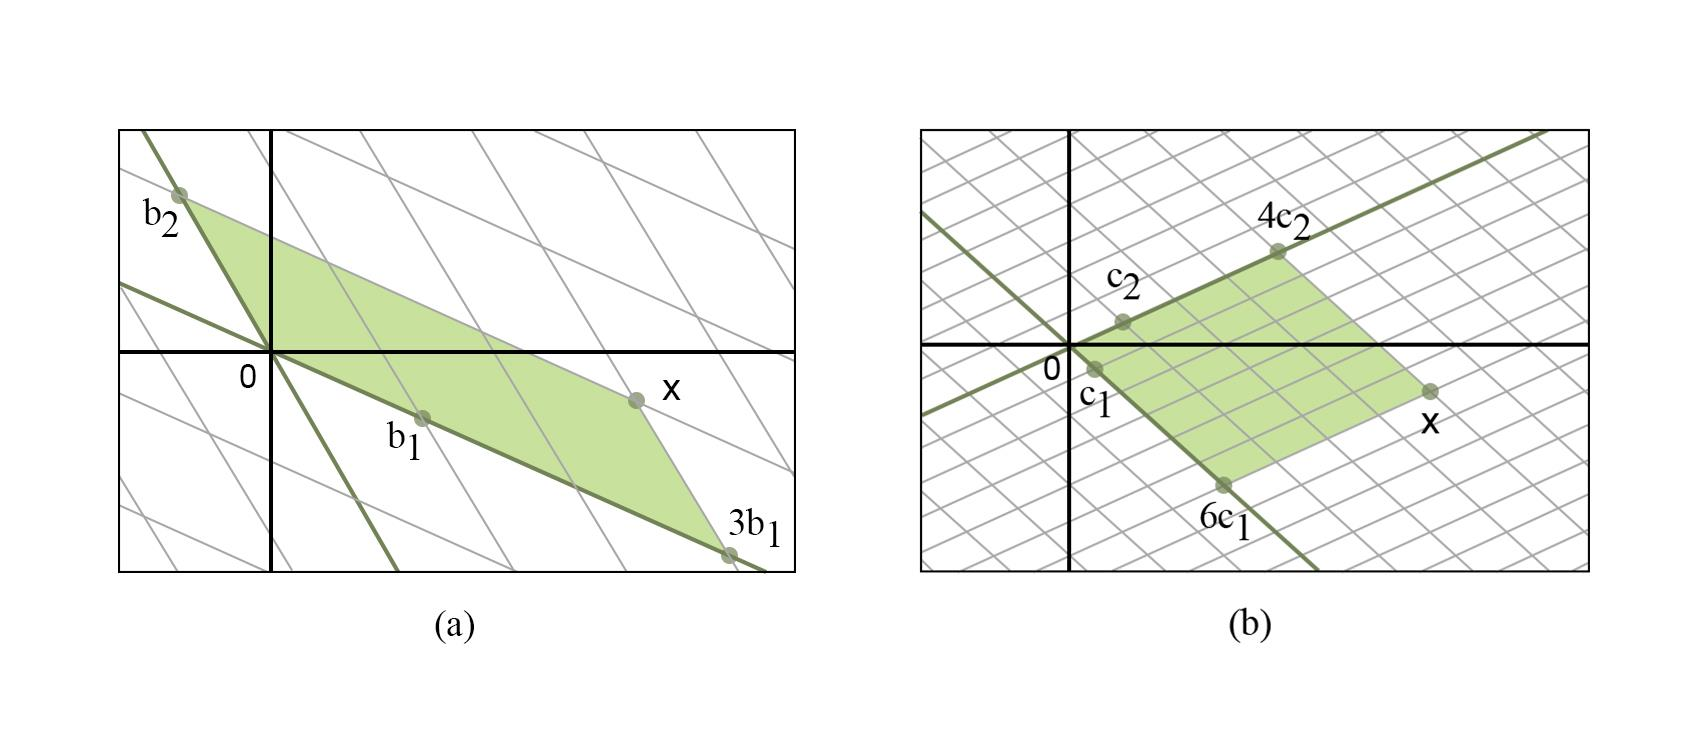
\includegraphics[width=0.99\textwidth]{Pictures/TLfig80.jpg}
    \caption{Coordenadas de un vector $\vec x$, en las bases $\{\vec b_1,\vec b_2\}$ (a) y $\{\vec c_1,\vec c_2\}$ $(b)$}
    \label{TLfig700}
\end{figure}


Para visualizar el problema de cambio de base, considere los dos  sistemas de  coordenadas que se muestran en
la Figura \ref{TLfig700}.  En $(a)$, $\vec{x} = 3\vec{b}_1 +1 \vec{b}_2$, mientras que en $(b)$, el mismo vector $\vec{x}$ se
expresa como $\vec{x} = 6\vec{c}_1 +4 \vec{c}_2$. 
%Esto es,
%[ x ]B = 3
%1
%y [ x ]C = 6
%4
El problema consiste en encontrar la relación que hay entre las coordenadas de un mismo vector $\vec{x}$ en las dos bases  $  \{\vec{b}_1,\vec{b}_2 \}$  y $  \{\vec{c}_1,\vec{c}_2 \}$ .
%En el ejemplo 1 se muestra cómo hacer esto, suponiendo que ya se sabe cómo
%están formadas b1 y b2 a partir de c1 y c2.



Para el caso general, supongamos que se tienen dos bases  $B$ y $B ^{\prime}$ de un espacio vectorial $V$ de dimensión finita. Se verá que con la ayuda de una matriz se pueden obtener las coordenadas de un vector con respecto a una base de $V$ a partir de las coordenadas del vector en la  otra base. Llamaremos base antigua a la base $B$ y base nueva a la base $B ^{\prime}$.


Si $B =\left\{\vec{e_1},\vec{ e_2},\cdots, \vec{e_m}\right\}$ y $B ^{\prime}=\left\{\vec{e}^{\prime}_1,\vec{e} ^{\prime}_2,\cdots, \vec{e} ^{\prime}_m\right\}$ son dos bases de un espacio vectorial $V$ de dimensión $n$,
todo elemento de la base  $B ^{\prime}$   puede escribirse como combinación lineal de los elementos de la base $B$ :

\begin{equation} \label{matriz Acb}
\left\{ \begin{array} {ccl} 
                    \vec{e }^{\prime}_1&\ =&   a_{11}\vec{e}_1+a_{21}\vec{e}_2+\cdots +a_{n1}\vec{e}_n    \\
                     \vec{e }^{\prime}_2 &\ = &a_{12}\vec{e}_1+a_{22}\vec{e}_2+\cdots +a_{n2}\vec{e}_n  \\
										\cdots  \\
                    \vec{e }^{\prime}_n &\ =&a_{1n}\vec{e}_1+a_{2n}\vec{e}_2+\cdots +a_{nn}\vec{e}_n
                   \end{array}
           \right.
\end{equation}


\bigskip

\noindent
que en forma abreviada puede escribirse


$$\vec{e }^{\prime}_j=\sum^{n}_{i=1}a_{ij}\vec{e}_i, \qquad j=1, \cdots n$$

\begin{remark}
Puede escribirse en forma más concisa  usando convenio de Einstein (índice repetido indica suma)
$$  \vec{e }^{\prime}_j=a_{ij}\vec{e}_i, \qquad  j=1, \cdots n  $$
%\hfill$\blacktriangle$
\end{remark}

\bigskip


La nueva  base $B ^{\prime}$   se obtiene de la base $B$ mediante la siguiente matriz 



$$A=\left(\begin{array}{cccc} a_{11} & a_{12}&  \cdots & a_{1n} \\a_{21}  & a_{22} & \cdots & a_{2n}
\\  \cdots & \cdots  &  \cdots  & \cdots \\ a_{n1} & a_{n2} & \cdots & a_{nn}
\end{array}
 \right)$$
 \bigskip
\noindent
donde la $j$-ésima columna de $A$ son las coordenadas del vector $\vec{e }^{\prime}_j$ con respecto a la base antigua $\vec{e}_j$, $j=1,2,\cdots ,n$.

\bigskip

 La matriz $A$ se denomina \textsl{matriz del cambio de base}  de   $B ^{\prime}$ a $B$ y se denota $P_{B, B^{\prime}}$.

\begin{remark}
\begin{itemize}
\item
A la matriz del cambio de base  de   $B ^{\prime}$ a  $B$ también se la denomina  \textsl{matriz de transición}  de la base   $B ^{\prime}$ a la base  $B$.
\item
 Cuando  sea necesario hacer constar las bases $B$ y $B ^{\prime}$ escribiremos $P_{B^{\prime},B}$ para denotar la matriz de cambio de base de  $B$ a $B ^{\prime}$. 

\item
Si $B$ y $B ^{\prime}$ coinciden se tiene que $P_{B ^{\prime},B}=I_{n {\times}n}$.
\end{itemize}
%\hfill$\blacktriangle$
\end{remark}



\begin{theorem}
\label{2141}
La matriz $A$ del cambio de base de  $B ^{\prime}$  a $B$  es invertible  y su inversa es la matriz de cambio de base de $B$ a  $B ^{\prime}$. Podemos,  por lo tanto, escribir

$$A^{-1}=P_{B,B ^{\prime}}^{-1}= P_{B ^{\prime},B}$$

\begin{proof} 

\noindent 
El determinante de la matriz es no nulo, ya que sus columnas son las coordenadas de los vectores $ \vec{e }_j $ que por ser una base son linealmente independientes.

\bigskip




Si  $A^{\prime}$ es la matriz de cambio de base de $B$ a $B^{\prime}$, entonces  se tiene 


$$\vec{e }_j=\sum^{n}_{i=1}a_{ij}^{\prime} \vec{e}^{\prime}_i, \qquad j=1, \cdots n$$

 


\bigskip
\noindent
 y por la definición de la matriz $A$,

 $$\vec{e }^{\prime}_i=\sum^{n}_{k=1}a_{ki} \vec{e}_k, \qquad i=1, \cdots n.$$
\noindent 
 por lo tanto, 

 \bigskip
 
$\vec{e }_j=\sum^{n}_{i=1}a_{ij}^{\prime} (   \sum^{n}_{k=1}a_{ki} \vec{e}_k)=\sum^{n}_{k=1}  (   \sum^{n}_{k=1}a_{ki}   a_{ij}^{\prime} ) \vec{e}_k, \qquad j=1, \cdots n.$


\bigskip


\noindent 
Como el término dentro de la sumatoria en $k$, $ \sum^{n}_{k=1}a_{ki}   a_{ij}^{\prime} $, es el elemento que ocupa el lugar $(k,j)$ del producto de las matrices $A$ y $A^{\prime}$,  de acuerdo a la igualdad, ese término   vale $1$ si $k=j$, y $0$ si no. Es decir que se tiene que el producto de las matrices  $A$ y $A^{\prime}$, es   $AA^{\prime}=I_{n \times n}$.

\end{proof}
\end{theorem}

\bigskip


\bigskip

\begin{remark}

\begin{itemize}



\item
Las expresiones anteriores pueden reescribirse en forma sintética  considerando que el índice repetido se suma de $1$ a $n$: 
$ \vec{e }_j=  a_{ij}^{\prime}  \vec{e}_i^{\prime}$

\bigskip

\item
Usando la delta de Kronecker,  $ \delta_{kj}$ (definida  $ \delta_{kj}=1$ si $k=j$ y $ \delta_{kj}=0$ si $k\neq j$),

\noindent
la expresión se escribe $ \vec{e }_j=a_{ki}  a_{ij}^{\prime}  \vec{e}_k= \delta_{kj}\vec{e}_k$
\end{itemize}
%\hfill$\blacktriangle$
\end{remark}


\bigskip


\begin{example}
\label{cambiob1}
Dadas las bases de  $\mathbb{R}^{3}$, $B =\left\{(1,1,1), (1,1,0),(1,0,0)\right\}$ y $B^{\prime}= \left\{\vec{e}_1,\vec{e}_2, \vec{e}_3\right\}$  (base canónica), la matriz de cambio de base de $B$ a $B^{\prime}$,  de acuerdo a las Ecs.(\ref{matriz Acb}), es


%\vskip1.25cm

$$P_{B ^{\prime},B}=\left(\begin{array}{ccc} 1 & 1 &  1 \\ 1 & 1 & 0
\\ 1 & 0 & 0
\end{array}
 \right)$$
\end{example}

\begin{remark}
\label{cambiobasecan}
Si la base nueva, $B^{\prime}$ es la base la canónica, la matriz de cambio de base de $B$ a $B^{\prime}$ se obtiene directamente  poniendo las coordenadas de los vectores de la base $B$ en cada columna  (ver Ejemplo \ref{cambiob1}).
%\hfill$\blacktriangle$
\end{remark}




\textbf{Relación entre las coordenadas en la base $B$ y en la $B^{\prime}$}
\label{RELCOORD}

\bigskip

\noindent 
Tratemos ahora de relacionar entre sí las coordenadas de un mismo vector en las bases nueva $B ^{\prime}$  y antigua $B$. Supongamos que $\vec{x}\in V$,


    
\begin{equation}
\label{ecx}
\vec{x}= x_1\vec{e}_1+x_2\vec{e}_2+\cdots +x_n\vec{e}_n 
\end{equation}

\noindent 
y además
\begin{equation}
\label{ecxp}
\vec{x}= x^{\prime}_1\vec{e}^{\prime}_1+x^{\prime}_2\vec{e}^{\prime}_2+\cdots +x^{\prime}_n\vec{e}^{\prime}_n 
\end{equation}

\bigskip

\noindent 
Sustituyendo Ec.(\ref{matriz Acb}) en la segunda expresión, Ec.(\ref{ecxp}), obtenemos

\bigskip

$$\vec{x}= x_1^{\prime} ( \sum^{n}_{i=1}  a_{i1} \vec{e}_i)+x_2^{\prime}( \sum^{n}_{i=1}  a_{i2} \vec{e}_i)+\cdots +x_n^{\prime}( \sum^{n}_{i=1}  a_{in} \vec{e}_i)$$

\bigskip

$$=(a_{11}x_1^{\prime}+  a_{12}x_2^{\prime}  +\cdots + a_{1n}x_n^{\prime}  )\vec{e}_1+ (a_{21}x_1^{\prime}+  a_{22}x^{\prime}_2  +\cdots$$


$$+ a_{2n}x_n^{\prime}  )   \vec{e}_2+\cdots +   (a_{n1}x_1^{\prime} +  a_{n2}x_2^{\prime}   +\cdots + a_{nn}x_n^{\prime}   )\vec{e}_n$$

\bigskip


Comparando esta última igualdad con la primera expresión Ec.(\ref{ecx}) podemos escribir 

\begin{equation} \label{ec4}
\left\{ \begin{array} {ccl} 
                    x_1&\ =&   a_{11}x_1^{\prime}+a_{12}x_2^{\prime}+\cdots +a_{1n}x_n^{\prime}    \\
                     x_2 &\ = &a_{21}x_1^{\prime}+a_{22}x_2^{\prime}+\cdots +a_{2n}x_n^{\prime}  \\
										\cdots  \\
                    x_n &\ =&a_{n1}x_1^{\prime}+a_{n2}x_2^{\prime}+\cdots +a_{nn}x_n^{\prime}
                   \end{array}
           \right.
\end{equation}

%\vskip1.25cm

Si convenimos en escribir $X=\left(\begin{array}{c} x_{1} \\ x_{2}  
\\  x_3 \\ \cdots \\ x_{n} 
\end{array}
 \right)$ y $X^{\prime}=\left(\begin{array}{c} x^{\prime}_{1} \\ x^{\prime}_{2}  
\\  x^{\prime}_3 \\ \cdots \\ x^{\prime}_{n} 
\end{array}\right)$ 

\bigskip
\noindent
a las coordenadas del vector $\vec{x}$ en la antigua base  $B$  y en la nueva base $B ^{\prime}$ , respectivamente, las Ecs.(\ref{ec4}) se escribe  de la forma

%\vskip1.25cm
\begin{equation}
\label{XPAX}
X=AX^{\prime}
\end{equation}

Esto  permite obtener las coordenadas del vector $\vec{x}$ en la base antigua  conociendo las coordenadas del mismo vector en la  base nueva.

%\vskip1.25cm



\begin{example}


Dadas las mismas  bases del Ejemplo \ref{cambiob1}, 

$B =\left\{(1,1,1), (1,1,0),(1,0,0)\right\}$ y $B^{\prime}= \left\{\vec{e}_1,\vec{e}_2, \vec{e}_3\right\}$, se quieren encontrar las coordenadas del vector $\vec{x}=(3,2,3)_{B^{\prime}}$ en la base $B$, para lo cual se necesita la matriz de cambio de base, $P_{B,B ^{\prime}}$.

De acuerdo a las Ecs. (\ref{matriz Acb}), la matriz de cambio de base, $P_{B,B ^{\prime}}$ se obtiene a partir de encontrar las coordenadas de  los vectores de la base $B^{\prime}$ en la base $B$  y colocarlos como columnas. Después de resolver el sistema de ecuaciones se obtuvo



\begin{equation} \label{ec5}
\left\{ \begin{array} {ccl} 
                   (1,0,0)&\ =&   0 (1,1,1)+0(1,1,0)+1(1,0,0)   \\
									(0,1,0)&\ =&   0 (1,1,1)+1(1,1,0)+(-1)(1,0,0)   \\
									(0,0,1)&\ =&   1 (1,1,1)+(-1)(1,1,0)+0(1,0,0)
                    \end{array}
           \right.
\end{equation}

\bigskip
\noindent
y entonces, 

\bigskip

$$P_{B,B ^{\prime}}=\left(\begin{array}{ccc} 0 & 0 &  1 \\ 0 & 1 & -1
\\ 1 & -1 & 0
\end{array}
 \right)$$
 
\bigskip

 Otra alternativa para hallar la matriz $P_{B,B ^{\prime}}$   es usar la Proposición \ref{2141} y entonces  $  P_{B,B ^{\prime}} = P_{B ^{\prime},B}^{-1}$ dado que $P_{B ^{\prime},B}$ se encontró en el Ejemplo \ref{cambiob1}.

\bigskip

Luego, usando (\ref{XPAX}), las coordenadas son

\bigskip

$$X=P_{B,B ^{\prime}}X^{\prime}=\left(\begin{array}{ccc} 0 & 0 &  1 \\ 0 & 1 & -1
\\ 1 & -1 & 0
\end{array}
 \right) \left(\begin{array}{c} 3 \\ 2  
\\ 3  
\end{array} \right)_{B ^{\prime}} =\left(\begin{array}{c} 3 \\ -1 
\\ 1  
\end{array} \right)_{B}$$

\bigskip

Así se obtuvieron  las coordenadas del vector $\vec{x}$ en la base  $B$ conociendo las coordenadas del mismo vector en la base $B ^{\prime}$.
\end{example}


\bigskip


\bigskip

\begin{example}
\label{ejrotR2}

Sean $\vec{e}_1$ y $\vec{e}_2$ dos vectores perpendiculares unitarios en $\mathbb{R}^{2}$ en la dirección de los ejes de coordenadas cartesianas. Girando los ejes de coordenadas un ángulo $\phi$ en sentido positivo, contrario a las agujas del reloj, se obtiene una nueva base  $B ^{\prime}=\{ \vec{e}_1^{\prime}$, $\vec{e}_2^{\prime}\}$.

\bigskip


\bigskip

De acuerdo a la Figura \ref{EVrot}, se observa que 


\begin{equation} \label{rot}
\left\{ \begin{array} {ccl} 
                    \vec{e}^{\prime}_1&\ =&   cos(\phi)\vec{e}_1+sen(\phi)\vec{e}_2    \\
                     \vec{e}^{\prime}_2 &\ = &-sen(\phi)\vec{e}_1+ cos(\phi)\vec{e}_2 \\
										
                   \end{array}
           \right.
\end{equation}

\bigskip
\noindent
por lo cual, teniendo en cuenta el sistema (\ref{matriz Acb}),  la matriz del cambio de base $A$ es 


\begin{equation}
\label{matrizrotR2}
A= \left(\begin{array}{cc}  cos(\phi) & -sen(\phi)  \\ sen(\phi) &  cos(\phi)
\end{array}
 \right)
\end{equation}

\begin{figure}
    \centering
    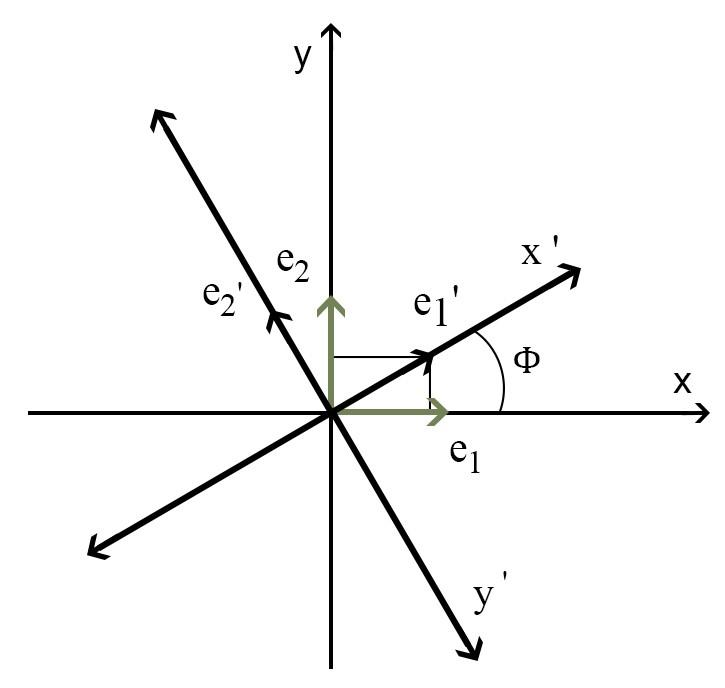
\includegraphics[width=0.60\textwidth]{Pictures/EVrot.jpg}
    \caption{Cambio de base. Rotación de ejes en un ángulo $\phi$.}
    \label{EVrot}
\end{figure}

\bigskip

Así, si $\phi= \pi/4$, las coordenadas respecto a la base $B=\{ \vec{e}_1^{\prime}$, $\vec{e}_2^{\prime} \}$ del vector $(2,3)_B$

\bigskip


$$\left(\begin{array}{cc}  cos(\pi/4) & -sen(\pi/4)  \\ sen(\pi/4) &  cos(\pi/4)
\end{array}
 \right)^{-1}\left(\begin{array}{c}  2 \\ 3
\end{array}
 \right)_{B}\approx \left(\begin{array}{c}  3.53 \\ 0.71
\end{array}
 \right)_{B ^{\prime}} $$
\end{example}


\bigskip

\bigskip

\begin{example}
Dadas las bases de $P_\mathbb{R}^{(2)}\left[x\right]$, $B =\left\{3,1+x,x^{2}\right\}$  y $B^{\prime}= \left\{1,x+3,x^{2}+x\right\}$, se quiere hallar la matriz de cambio de base de $B ^{\prime}$ a $B$.

Teniendo en cuenta la Observación {\textcolor{blue}{\fontfamily{qcr}\selectfont{i}}}, luego del Ejemplo \ref{cambiob1} resulta más simple hallar $P_{E,B}$ y  $P_{E,B ^{\prime}}$, donde $E =\left\{1,x,x^{2}\right\}$ es la base canónica.
 Como 


\begin{eqnarray*}
1&= & 1\cdot 1+0 \cdot x+ 0 \cdot x^2 \\
x+3&= &3\cdot1+ 1\cdot x +  0\cdot x^2 \\
x^2+x & = &0\cdot 1+ 1\cdot x + 1\cdot x^2
\end{eqnarray*}

Se tiene  que  
$$P_{E,B ^{\prime}}=\left(\begin{array}{ccc} 1 & 3 &  0 \\ 0 & 1 & 1
\\ 0 & 0 & 1
\end{array}
 \right)$$ 
 \bigskip
 \noindent
 y de la misma forma, 
$$P_{E,B}=\left(\begin{array}{ccc} 3 & 1 &  0 \\ 0 & 1 & 0
\\ 0 & 0 & 1
\end{array}
 \right)$$


\bigskip


Luego, la matriz de cambio de base de $B ^{\prime}$ a $B$ sale de multiplicar  las matrices de cambio de base de $E$ a $B$ y de $ B ^{\prime}$ a $E$, es decir,

$$P_{B,B ^{\prime}}=P_{B,E}P_{E,B ^{\prime}}=(P_{E,B})^{-1}P_{E,B ^{\prime}}= \left(\begin{array}{ccc} 1/3 & 2/3 &  -1/3 \\ 0 & 1 & 1
\\ 0 & 0 & 1
\end{array}
 \right)$$

\bigskip

$\left(\begin{array}{ccc} 1/3 & 2/3 &  -1/3 \\ 0 & 1 & 1
\\ 0 & 0 & 1
\end{array}
 \right)\left(\begin{array}{c} 0 \\ 0  
\\ 1 
\end{array} \right)_{B^{\prime}}=\left(\begin{array}{c} -1/3\\ 1  
\\ 1 
\end{array} \right)_B =x^{2}+x $

\end{example}














%\begin{VF}
%``A Process is a structured, measured set of activities designed to produce a specific output for a particular customer
%or market---A process is thus a specific ordering of work activities across time and space, with a beginning, an end.
%and clearly defined inputs and outputs: a structure for action.''%

%\VA{Thomas Davenport}{Senior Adjutant to the Junior Marketing VP}
%\end{VF}













\index{Goobar, Ariel}
\begin{parchment}[Ariel Goobar]{Nacido en Argentina en 1962, Es un astrofísico sueco que trabaja en la Universidad de Estocolmo en astrofísica de altas energías y teoría de la relatividad. Es integrante del equipo que ganó el Nobel de Física en 2011 por descubrir mediante las mediciones con supernovas, la expansión acelerada del universo, actualmente es Director del Oskar Klein Centre for Cosmoparticle Physics. Emigró de Argentina a los 13 años. Se dedica al contenido de lo que se llama materia oscura.
La gran esperanza –aunque a lo mejor me equivoco dijo– desde el punto de vista experimental es que si entendemos qué es la energía oscura, muy probablemente eso nos vaya a dar un indicio importante de cómo se puede entender la fuerza de gravedad, cómo casar la teoría de la relatividad con la física cuántica. Muy probablemente estén relacionadas, pero hoy no tenemos idea de cómo. Hoy, si yo pudiera soñar algo, creo que es entender eso, sería alucinante. \cite{goobar}}
\end{parchment}















\bigskip


\newpage



%\begin{figure}
%\label{figproyxy}
 %   \centering
    %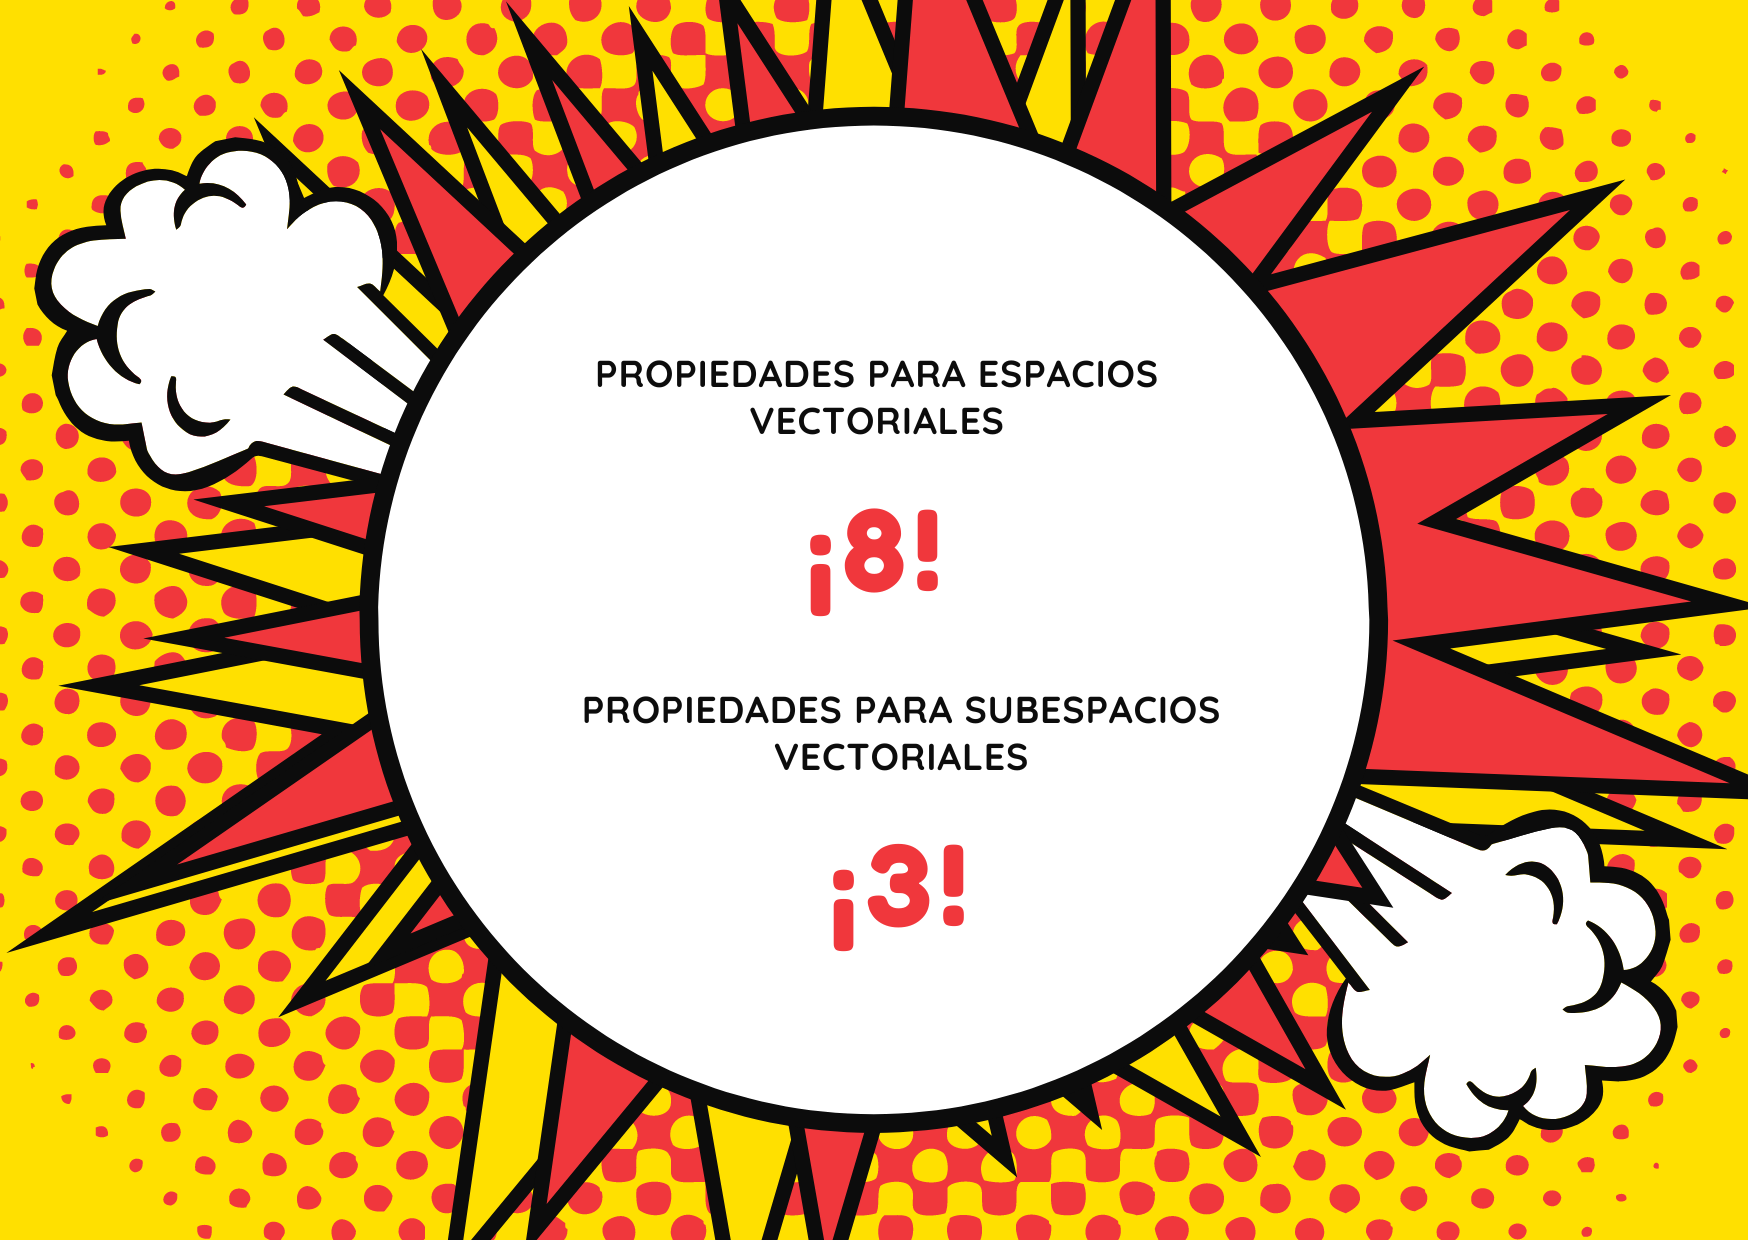
\includegraphics[width=0.60\textwidth]{Pictures/8.png}    
   % \label{TLfig10}
%\end{figure}




\section{Actividades propuestas}
%\subsection{}
\begin{answers}
Para realizar un cambio de coordenadas celestes a coordenadas horizontales\index{Cambio de coordenadas celestes}, es necesario hacer dos rotaciones:


\begin{figure}
    \centering
    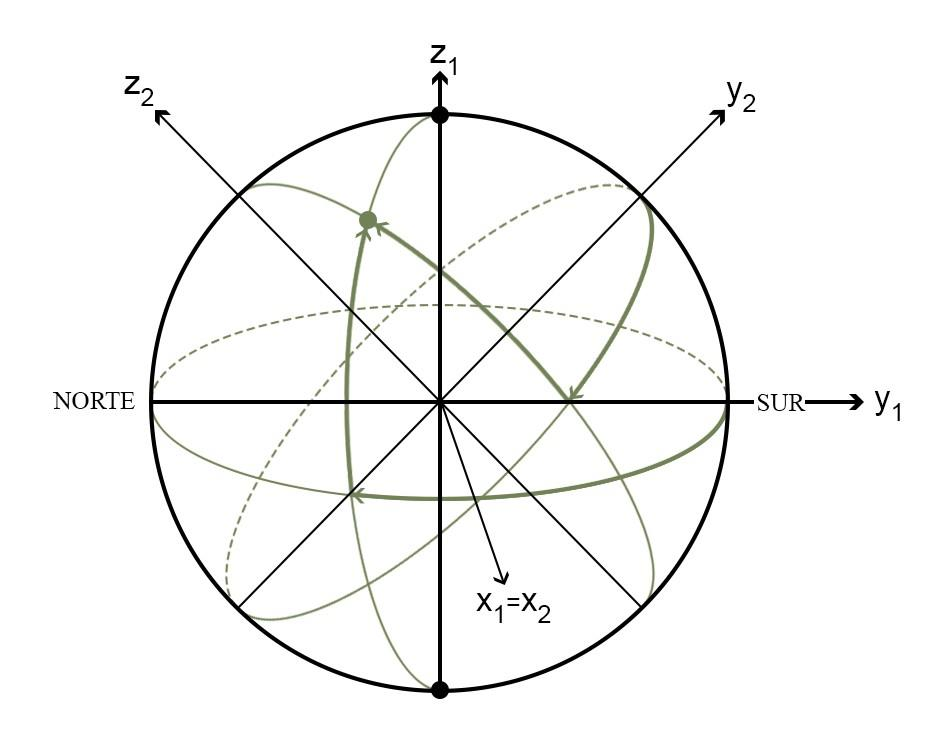
\includegraphics[width=0.7\textwidth]{Pictures/fig.42.jpg}
    \caption{Coordenadas $(x_1, y_1, z_1)$ y $(x_2, y_2, z_2)$ en el sistema cartesiano  horizontal y en el cartesiano  ecuatorial}
%horario respectivamente}
    \label{Esfera}
\end{figure}
%Figura nueva si se denotan con (x1, y1, z1) y (x2, y2, z2) las coordenadas de un astro en el
%sistema cartesiano tridimensional horizontal y en el cartesiano tridimensional ecuatorial
%horario respectivamente, teniendo en cuenta la definición de ambos sistemas, se
%obtienen por:

%\textcolor{red}{revisar fórmula no se aclara que son subindices  h, el y ec ? abajo si aclaro que son y como se escriben }

$$\vec{r}_{el}= R_z(TSL)*\vec{r}_{ec}$$

$$\vec{r}_{h}= R_y(90-\varphi)*\vec{r}_{el}$$

Esto se debe a que entre el sistema ecuatorial celeste y el ecuatorial local, el polo celeste (eje $z$) permanece  fijo para ambos, pero el origen desde donde medimos uno y otro sitema en el ecuador celeste, cambia en una cantidad TSL. Usaremos $TSL$ como tiempo siderio local, $TSL$= 18:31:31, Recuerde pasar de horas a grados para poder operar. Luego para realizar el cambio de coordenadas de celeste locales a horizontales, se mantiene en común el eje $y$, la línea este-oeste, y el ángulo en que se rotan el plano $x$, $z$ es $90-\varphi$. Para el problema actual usaremos la $\varphi$= $-$34º 50'  que corresponde a la ciudad de La Plata.

\bigskip

%\textcolor{red}{no entiendo la primera frase por qué entre, la reescribi pero tengo dudas. puse comas, revisar }

%\textcolor{red}{Esto se debe a que entre el sistema ecuatorial celeste y el sistema ecuatorial local, el polo celeste (eje $z$) permanece  fijo para ambos, pero el origen desde donde medimos uno y otro sistema en el ecuador celeste, cambia en una cantidad TSL. Usaremos $TSL$ como tiempo siderio local   $TSL= 18:31:31$, 
%Luego, para realizar el cambio de coordenadas de celestes locales a horizontales, se mantiene en común el eje $y$, la línea este-oeste, y el ángulo en que se rotan el plano $x$, $z$ es $90-\varphi$. Para el problema actual utilice  $\varphi= -34º 50'$,  que corresponde a la ciudad de La PLata. Creo haber agregado las comas ect..}

\bigskip

El vector de las coordenadas ecuatoriales celestes se escribe como:

\bigskip

$$\vec{r}_{ec}=\left(\begin{array}{c} cos(\delta)cos(\alpha)\\cos(\delta)sen(\alpha) \\ sen(\delta)
\end{array}
 \right)$$

 
\bigskip
\noindent
y el vector de las coordenadas horizontales:

$$\vec{r}_{h}=\left(\begin{array}{c} cos(h)cos(A)\\-cos(h)sen(A) \\ sen(h)
\end{array}
 \right)$$

 \bigskip
 
\noindent
donde $h=sen^{-1}(z)$ y $A=tan^{-1}(-y/x)$.

\bigskip
 
 Amplíe la Tabla \ref{cum} con las coordenadas horizontales para cada cúmulo.  Recuerde pasar de horas a grados para poder operar. Nota: No tenga en cuenta la precesión. \textcolor{blue}{Recomendación}: Realice un programa computacional para hacer los cálculos.

 
 \bigskip

%\end{document}

\begin{table}
%[!hbt]
\renewcommand{\tablename}{Tabla}
\centering
\begin{tabular}{L{0.15\textwidth} R{0.15\textwidth} R{0.15\textwidth}} 
%Specify column alignment with L{width}, C{width} and R{width} for fixed-%width columns, or the default latex l, c and r for flexible-width columns
		\toprule
		\textbf{Cúmulo} & \textbf{RA(J2000)} & \textbf{Dec(J2000)}\\%
		\midrule
NGC6192 &16:40:16.40 & $-$43:30:31.0\\
NGC6242 & 16:55:32.38& $-$39:28:02.0\\
NGC6322&17:18:25.13  & $-$42:56:03.3\\
NGC6704 &18:50:42.00 & $-$05:12:42.5\\
NGC6737 &19:02:16.30 & $-$18:32:56.5\\
Rup 102 & 12:13:32.95& $-$62:43:18.7\\
Rup 166 & 13:25:38.14& $-$63:27:54.6\\
SLS4565& 18:01:59.55&$-$23:41:06.3\\
Lynga 14& 16:55:03.40&$-$45:14:09.1\\
Trumpler 22& 14:31:03.33&$-$61:09:57.0\\
Trumpler 24& 16:56:11.14&$-$40:40:01.1\\
Dominici 11& 18:57:36.31&$-$10:23:39.9\\
Dominici 12& 18:51:24.93&$-$13:18:50.2\\
\bottomrule
\end{tabular}
\caption{Coordenadas celestes de 13 cúmulos abiertos.}
\label{cum} % Unique label used for referencing the table in-text
\end{table}

 


\end{answers}

\bigskip

 \bigskip

 

\subsection{Ejercicios}

%\subsubsection{Espacios Vectoriales. Subespacios. Suma de subespacios.}

 

%\newpage
\begin{exercise}
\item
Analice si los siguientes conjuntos son espacios vectoriales
sobre $\mathbb{R}$. 
%(asumiendo que $\oplus$ y $\ast$ son las operaciones naturales)

a) El conjunto  $S=\{(x,y) : y=2x+1\}
\subseteq \mathbb{R}^2$

b) El semiplano en $\mathbb{R}^2$,  $S=\{(x,y) : y\geq 0\}$, 

c) Los polinomios de grado menor o igual que 2, $P^{(2)}_{\mathbb{R}}[x]$.

\end{exercise}



\begin{exercise}
\item
Dé al menos $5$ ejemplos de espacios vectoriales y escriba según su opinión, 
qué utilidad podría tener saber que tienen estructura de espacio vectorial.
\end{exercise}
\begin{exercise}
\item 

De acuerdo con la definición; $S$ es un subespacio de un espacio vectorial $V$ sí 
y sólo sí, se cumplen las siguientes condiciones:

i) S contiene al vector $\vec{0}$ de $V$.

ii) Si $\vec{u}$ y $\vec{v}$ están en S, entonces $\vec{u}$  + $\vec{v}$ está en $S$.

iii) Si $\vec{u}$ está en $S$ y $\alpha$ es un escalar entonces, $\alpha\vec{u}$ está en $S$.

\noindent Compruebe si valen las siguientes afirmaciones:

\noindent a) $S=\{(x,y,z) : z=0\}$, es un subespacio de $\mathbb{R}^3$.

\noindent b) El conjunto de polinomios $P^{(2)}_{\mathbb{R}}[x]$, de grado menor o igual que $2$, es subespacio vectorial del espacio vectorial 
$P^{(n)}_{\mathbb{R}}[x]$ de todos los polinomios con coeficientes reales.


\end{exercise}

%\bigskip

\begin{exercise}
\item

Dados los subespacios de $\mathbb{R}^3$, $S$=$\{(x,y,z)\in \mathbb{R}^3: x=y=0\}$ y
$T=\{(x,y,z) \in \mathbb{R}^3: x+y+z=0\}$ calcule:
a) Una base y la dimensión de ambos subespacios.
b)  $S + T$ y $ S \cap T$, dando las bases de dichos subespacios.
c) ¿La suma $S + T$ es directa?
\end{exercise}

\begin{exercise}
\item

Encuentre en cada uno de los ejemplos siguientes la suma y la intersección del par de subespacios dados, y compruebe
que se verifica la ecuación:

\bigskip

    $dim(V_1)+dim(V_2) = dim(V_1+V_2) + dim(V_1 \cap V_2)$
    
\bigskip
		
		
a) Siendo el conmutador la diferencia entre $A.B - B.A$ con $A$ y $B$ matrices, y trabajando con que el conmutador sea necesariamente la matriz nula, encuentre los subespacios que se forman si $A$ es la matriz que se muestra en cada caso:

\bigskip

$A_1=\left(\begin{array}{cc} 2 & 1  \\ 0 & 2 
\end{array}
 \right), \qquad    A_2=\left(\begin{array}{cc} 2 & 0 \\ 1 & 2 
\end{array}
 \right)$\\
 
 \bigskip
 
b) Los subespacios formados por las bases $\{sen(t),cos(t)\}$ y $\{e^{it},e^{-it}\}$ considerados en el espacio real de las funciones complejas continuas en el intervalo $[0,1]$.
\end{exercise}

 
\begin{exercise} 
\item
 \begin{enumerate}
 
 \item 
 Demuestre que el conjunto de soluciones de la ecuación diferencial de primer orden homogénea, con coeficientes constantes:
 $y' + k y=0$ es un espacio vectorial de dimensión uno, siendo $\{e^{-kx}\}$ una base. A su vez el conjunto de soluciones de esta ecuación
 es un subespacio vectorial del espacio de las funciones derivables cuya dimensión es infinita.

\bigskip 
    
 
\item  Luego resuelva la ecuación diferencial homogénea de segundo orden:
 
 $y''- y' - 6y=0$, con las condiciones iniciales y(0)=3
 y y'(0)=-1.\\
 
  Dado que éste tipo de ecuaciones se resuelve usando la ecuación característica, que para éste caso sería:
 $\lambda^2-\lambda-6=0$.
 \begin{enumerate}
   
 \item Encuentre las raíces $\lambda_1$ y $\lambda_2$ y reemplazar en la función: $y(x)= C_1e^{\lambda_1 x}+C_2e^{\lambda_2 x}$.
 
 \item Escriba la base del conjunto solución, y especifique que dimensión tiene. 
 \item Halle la solución particular definiendo los coeficientes $C_1$ y $C_2$, con ayuda de las condiciones iniciales.
 \end{enumerate}
 \item Averigue que pasaría si las soluciones de la ecuación característica de una ecuación diferencial homogénea fueran raíces dobles. Escriba su base.
 
\item Cite al menos un ejemplo de física donde se necesita usar ecuaciones diferenciales.
\end{enumerate}
\end{exercise}

\begin{exercise}
\item

¿Son los vectores  $\vec{u}=(4,-2,5)$ y $\vec{v}=(1,-1,-1)$ de $\mathbb{R}^3$ combinación lineal
de $\vec{x_1}=(1,-1,2)$ y $\vec{x_2}=(2,0,1)$? Interprete geométricamente y conecte con los subespacios de 
$\mathbb{R}^3$.
\end{exercise}

\begin{exercise}
\item

Los primeros cuatro polinomios de Laguerre son  $\{1, 1-x, 2-4x+x^2, 6-18x + 9x^2 - x^3\}$. Demuestre que estos polinomios forman una base de $P^{(3)}_{\mathbb{R}}[x]$.
\end{exercise}

\begin{exercise}
\item

Compruebe que $B=\{1,x,x^2\}$ es una base del espacio vectorial $P^{(2)}_{\mathbb{R}}[x]$. En consecuencia dim$(P^{(2)}_{\mathbb{R}}[x])$= 3.
¿Es correcta la afirmación dim$(P^{(n)}_{\mathbb{R}}[x])$= n+1?
 \end{exercise}
\begin{exercise}
\item

Sea la matriz, 


$$A=\left(\begin{array}{ccc}x & a & b \\ a & x & b\\ a & b & x 
\end{array}
 \right)$$

 \bigskip
\noindent 
Encuentre los valores de $x$ para los que el $Det (A)= 0$. Lo cual es equivalente a decir que columnas o filas son linealmente dependientes.
¿Cuáles son las dimensiones posibles del espacio generado por las filas?

\end{exercise}





%\subsubsection{Bases. Coordenadas de  un vector en una base. Cambio de base.}


 
\begin{exercise}
\item

Encuentre las coordenadas del vector  $\vec{x}=(1,3,-2)$ con respecto a la base B=$\{\vec{b_1}, \vec{b_2}, \vec{b_3}\}$
donde $\vec{b_1}=(1,0,0)$, $\vec{b_2}=(1,1,0)$, $\vec{b_3}=(1,1,1)$.

\bigskip

\end{exercise}

\begin{exercise}
\item
 Calcule las coordenadas del vector $\vec{w}$ relativas a la base
$B=\{ \vec{u}_1,\vec{u}_2\}$.

a) $\vec{u}_1=(1,0)$, $\vec{u}_2=(0,1)$; $\vec{w}=(3,7)$

b) $\vec{u}_1=(2,-4)$, $\vec{u}_2=(3,8)$; $\vec{w}=(1,1)$

c) $\vec{u}_1=(1,1)$, $\vec{u}_2=(0,2)$; $\vec{w}=(a,b)$\\

\end{exercise}

\begin{exercise}
\item
Encuentre las coordenadas del vector $\vec{v}$ relativas a la base $B=\{
\vec{v}_1,\vec{v}_2,\vec{v}_3\}$.

 $\vec{v}_1=(1,0,0)$, $\vec{v}_2=(2,2,0)$, $\vec{v}_3=(3,3,3)$; $\vec{v}=(2,-1,3)$.\\
\end{exercise}

\begin{exercise}
\item

Calcule las coordenadas del vector $p \in P^{(2)}_{\mathbb{R}}[x]$ relativas a la base $B=\{
p_1(x),p_2(x),p_3(x)\}$.



$p_1(x)=1+x$, $p_2(x)=1+x^2$, $p_3(x)=x+x^2$; $p(x)=4-3x+x^2$\\
\end{exercise}
\begin{exercise}
\item
En $\mathbb{R}^{2\times2}$, encuentre las coordenadas de la matriz
$A=\left(\begin{array}{cc}2 & 0  \\-1 & 3
\end{array}
 \right)$ relativas a la base


\[ B= \left\{
 \left(\begin{array}{cc}-1 & 1  \\0 & 0
\end{array}
 \right),\left(\begin{array}{cc}1 & 1  \\0 & 0
\end{array}
 \right),\left(\begin{array}{cc}0 & 0  \\1 & 0
\end{array}
 \right),\left(\begin{array}{cc}0 & 0  \\0 & 1
\end{array}
 \right)
 \right \}
 \]\\
\end{exercise}
\begin{exercise}
\item 


Considere las bases $B=\{ \vec{u}_1,\vec{u}_2\}$  y $B^\prime=\{ \vec{v}_1,\vec{v}_2\}$ para
$ \mathbb{R}^2$, donde  $\vec{u}_1=(1,0)$, $\vec{u}_2=(0,1)$, $\vec{v}_1=(2,1)$,
$\vec{v}_2=(-3,4)$.

a) Halle la matriz de cambio de base de $B$ a $B^\prime$, $P_{B^\prime,B}$.

b) Utilice la matriz anterior para obtener las coordenadas en la base
$B^\prime$ de $\vec{w}=(3, -5)_{B}$.

c) Verifique lo obtenido en b) haciéndolo directamente.

d) Calcule la matriz de transición $P_{B,B^\prime}$ y verifique que
$P_{B,B^\prime}= P^{-1}_{B^\prime,B}$.
\end{exercise}

\begin{exercise}
\item

Considere las bases $B=\{ \vec{u}_1,\vec{u}_2, \vec{u}_3\}$  y $B^\prime=\{ \vec{v}_1,\vec{v}_2,
\vec{v}_3\}$ para $ \mathbb{R}^3$, donde  $\vec{u}_1=(-3,0,-3)$,
$\vec{u}_2=(-3,2,1)$, $ \vec{u}_3=(1,6,-1)$, $ \vec{v}_1=(-6,-6,0)$, $\vec{v}_2=(-2,-6,4)$ y
$\vec{v}_3=(-2,-3,7)$.\\

a) Halle la matriz de cambio de base de $B$ a $B^\prime$.


b) Utilice la matriz anterior para obtener las coordenadas en la base
$B^\prime$ de $\vec{w}=(-5, 8, -5)_{B}$.
\end{exercise}



\begin{exercise}
\item

Considere las bases $B=\{ p_1(x),p_2(x)\}$  y $B^\prime=\{ q_1(x),q_2(x)\}$ para
$P^{(1)}_{\mathbb{R}}[x]$, donde  $p_1(x)=6+3x$, $p_2(x)=10+2x$, $q_1(x)=2$, $q_2(x)=3+2x$.

a) Halle la matriz de transición de $B$ a $B^\prime$.

b) Utilice la matriz anterior para obtener las coordenadas de $p(x)=-4+x$
en la base $B^\prime$.\\
\end{exercise}
%\vspace{0.15cm}



\begin{exercise}
\item

Si se quiere obtener un sistema de coordenadas rectangulares
$x'y'$ haciendo girar un sistema de coordenadas rectangulares $xy$ hasta
describir un ángulo de $\theta= \frac {3 }{4} \pi$.

a) Halle las coordenadas $x^\prime y^\prime$ del punto cuyas coordenadas $xy$
son $(-2,6)$.

b) Calcule las coordenadas $xy$ del punto cuyas coordenadas $x^\prime y^\prime$
son $(5,2)$.

%\vspace{0.15cm}
\end{exercise}

\begin{exercise}
\item

Si se quiere obtener un sistema de coordenadas rectangulares
$x^\prime y^\prime z^\prime$ haciendo girar un sistema de coordenadas rectangulares $xyz$ en sentido
contrario a las agujas del reloj alrededor del eje $z$, cuando se
observa hacia abajo a lo largo del eje $z$ hasta describir un
ángulo de $\theta= \frac {\pi}{4}$.

a) Halle las coordenadas $x^\prime y^\prime z^\prime$ del punto cuyas coordenadas
$xyz$ son $(-1,2,5)$.

b) Calcule las coordenadas $xyz$ del punto cuyas coordenadas
$x^\prime y^\prime z^\prime$ son $(1,6,-3)$.

\end{exercise}



 %\subsection{Ejercicios teóricos}\\
 
\begin{exercise}
\item

Sea $V$ un espacio vectorial de dimensión $n$. Demuestre que todo conjunto linealmente independiente de $n$ elementos es una base de $V$.
\end{exercise}

\begin{exercise}
\item

Sean $p_0(x), p_1(x),.., p_n(x)$ polinomios cualesquiera de $P^{(n)}_{\mathbb{R}}[x]$ de grado $0,1,  \cdots,n$ respectivamente: demuestre que 
$\{p_0(x), p_1(x),..,p_n(x)\}$ es una base de $P^{(n)}_{\mathbb{R}}[x]$. ¿Podría encontrar alguna relación entre este teorema y el teorema del resto?
¿Y con la fórmula de Taylor?
\end{exercise}
\begin{exercise}
\item

En el supuesto que V=$V_1\oplus V_2$ donde $V_1$ y $V_2$ son dos subespacios de V de dimensiones n y m respectivamente y sean $B_1=\{\vec{u}_1,\vec{u}_2,\cdots,\vec{u}_n\}$ y $B_2=\{\vec{v}_1,\vec{v}_2,\cdots,\vec{v}_n\}$ sus bases, compruebe que $B=B_1 \cup B_2$ es una base de $V_1\oplus V_2$.
\end{exercise}

\bigskip


\bigskip

\begin{exercise}
\item
Sea $A=LU$, donde $L$ es una matriz triangular inferior invertible y $U$ es triangular superior. Explique por qué la primera columna de $A$ es un múltiplo de la primera columna de $L$. ¿Cómo se relaciona la segunda columna de $A$ con las columnas de $L$?\\
\end{exercise}



\begin{exercise}
\item
Sea $\{\vec{e_1},\vec{e_2},\cdots,\vec{e_n}\}$ la base canónica de $\mathbb{R}^n$, y sean $\vec{u_1}=\vec{e_2}- \vec{e_1}$, $\vec{u_2}=\vec{e_3}- \vec{e_2}, \cdots,  \vec{u_n}=\vec{e_{n}}- \vec{e_{n-1}}$. 
Demuestre que  $\{\vec{u_1},\vec{u_2},\cdots,\vec{u_n}\}$ es una base de $\mathbb{R}^n$.
Exprese el vector $ \vec{v} = \vec{e_1}+ \vec{e_2}+\cdots+\vec{e_n}$  como una combinación lineal de los vectores $\vec{u_1},\vec{u_2},\cdots,\vec{u_n}$.\\


\end{exercise}


%\newpage

\bigskip

 \subsection{Autoevaluación}
 \label{Auto1}
 

\subsubsection{Verdadero o Falso.}


 \bigskip

\begin{enumerate}

\item

Si una matriz tiene dos filas iguales, su determinate vale $0$.

\item

Si F= $F_1 \oplus F_2 \oplus .. \oplus F_p$ entonces dim F $ \neq $ dim $F_1$ + dim $F_1$ + .. + dim $F_p$.

\item

Si $P_{B,A}$ es invertible, entonces $P^{-1}_{B,A}$=$P_{B,A}$.

\item

Siendo $A$,$ B$ y $C$  bases de un espacio vectorial,  se cumple que $P_{C,B}.P_{B,A}$=$P_{C,A}$. 

\item

 Sea S un conjunto de un espacio vectorial V de dimensión n y además S contiene menos de n vectores, entonces S no puede generar V.

\item

Un plano en $\mathbb{R}^3$ es un subespacio de dimensión $2$ de $\mathbb{R}^3$.


\item

Si un conjunto $\{\vec{v_1},\vec{v_2},\cdots,\vec{v_p}\}$ genera un espacio vectorial V de dimensión finita y si T es un conjunto de más de p vectores en V, entonces T es linealmente dependiente.

\item

La suma del subespacio de  las matrices simétricas de $\mathbb{R}^{n \times n}$  con las matrices antisimétricas de $\mathbb{R}^{n \times n}$ es directa generando el espacio vectorial de las matrices de $\mathbb{R}^{n \times n}$.

\item

La suma del subespacio de las  funciones pares con el subespacio de las funciones impares no es directa.

\end{enumerate}

